
\documentclass[onecolumn,a4paper,11pt]{article}
\voffset -1cm
\hoffset -1cm
\textheight 22.3cm
\textwidth 15.0cm

\usepackage{blindtext}
%\usepackage{titlesec}
\usepackage[utf8]{inputenc}
\usepackage{times}
\usepackage{microtype}

\usepackage{lscape}

\setcounter{secnumdepth}{5}
\setcounter{tocdepth}{5}

\usepackage{epstopdf}

\usepackage{natbib}
\bibliographystyle{plainnat}
\bibpunct{(}{)}{;}{a}{,}{,}
\usepackage{subfigure}
\usepackage{multirow}
\usepackage{float}
\usepackage{soul}
\usepackage{xcolor}
\graphicspath{{./images/}}

\usepackage{amssymb}
\usepackage{amsmath}
\usepackage{mathtools}
\usepackage{amsthm}
\usepackage{bm}
\usepackage{url}
\usepackage{parskip}

\usepackage[titletoc]{appendix}
\usepackage{booktabs}
\usepackage{boldline}
\usepackage{colortbl}
\DeclareMathOperator{\LogNormal}{LogNormal}
\DeclareMathOperator{\GP}{\mathcal{GP}}
\DeclareMathOperator{\Normal}{Normal}

\providecommand{\keywords}[1]
{
  \small	
  \textbf{\textit{Keywords---}} #1
}


% \bibpunct[, ]{[}{]}{,}{}{,}{,}
\renewcommand\bibfont{\fontsize{10}{12}\selectfont}

\usepackage{listings}
\usepackage{slashbox}
\usepackage{caption}
\captionsetup{font=footnotesize}
\usepackage[colorlinks=true,citecolor=black,linkcolor=black,urlcolor=black]{hyperref}

%\bibliographystyle{authordate1}
% TODO macro
\newcommand{\todo}[1]{\textcolor{blue}{\textbf{[#1]}}}
\newcommand{\resp}[1]{\textcolor{red}{\textbf{[#1]}}}


\title{Online supplemental material of the article:\\ \vspace{7mm} 'Practical Hilbert space approximate Bayesian Gaussian processes for probabilistic programming'\\ \vspace{7mm}
\normalsize by}

\author{Gabriel Riutort-Mayol and Paul-Christian Bürkner and Michael R.\ Andersen and\\
  Arno Solin and Aki Vehtari}

\date{}


\begin{document}

\maketitle

This document consists of four case studies of application of the article 'Practical Hilbert space approximate Bayesian Gaussian processes for probabilistic programming'.

\tableofcontents

\appendix

\counterwithin{figure}{section}
\counterwithin{table}{section}
\counterwithin{equation}{section}

\section{Same-sex marriage case study}\label{ch5_sec_studycaseII}
This data set relates the proportion of support for same-sex marriage to the age. The data consists of 74 observations of the amount of people $y_i$ supporting same-sex marriage from a population $n_i$ per age group $i$ ($i=1,\dots,74$). The observational model is a binomial model with parameters population $n_i$ and probability of supporting same-sex marriage $p_i$ per age group $i$,
%
\begin{equation*}
y_i \sim \mathrm{Binomial}(p_i, n_i).
\end{equation*}

\noindent The population per age group $n_i$ is a known quantity and the goal is to estimate the same-sex support probability $p_i$ or mean number of support people per age group. Probabilities $\bm{p}=(p_1,\dots,p_{74})$ are modeled by a Gaussian process (GP) function $f:{\rm I\!R} \to {\rm I\!R}$ with a squared exponential covariance function $k$, as a function of age input values $\bm{x}=(x_1,\dots,x_{74})$, and through the {\it logit} function as a link function,
%
\begin{align*} \label{ch5_eq_gpprior_gay}
p_i &= \mathrm{logit}(f(x_i)) \nonumber \\
f(x) &\sim \mathcal{GP}(0, k(x,x', \theta)).
\end{align*}

\noindent Saying that the function $f(\cdot)$ follows a GP model is equivalent to say that $\bm{f}$ is multivariate Gaussian distributed with covariance matrix $\bm{K}$, where $K_{ij}=k(x_i,x_j,\theta)$, with $i,j=1,\dots,74$. The covariance function $k$ depends on the inputs $\bm{x}$ and hyperparameters $\theta=\{\alpha,\ell\}$. The hyperparameters $\alpha$ and $\ell$ represent the marginal variance and lengthscale, respectively, of the GP process.

In the HSGP model, the function $f(x)$ is approximated as in equation (7)%(\ref{eq_approxf})
, with the squared exponential spectral density as in equation (1)%(\ref{eq_specdens_inf})
, and eigenvalues $\lambda_j$  and eigenfunctions $\phi_j$ as in equations (5) %(\ref{eq_eigenvalue}) 
and (6)%(\ref{eq_eigenfunction})
. 

In order to do model comparison, in addition to the regular GP model and HSGP model, an splines-based model is also fitted using the Thin Plate Regression Splines approach in \cite{wood2003thin} and implemented in the R-package \textit{mgcv} \citep{wood2011mgcv}. A Bayesian approach is used to fit this splines model using the R-package \textit{brms} \citep{burkner2017brms}.

Figure \ref{ch5_fig12_Posteriors_gaydata} shows the posterior mean predictive distributions of the three models, the regular GP, the HSGP model with $m=20$ basis functions and boundary factor $c=1.5$, and the splines model with 20 knots. Sample observations are plotted as circles in the figure, and the out-of-sample observations, which have been used for testing, are plotted as crosses.

\begin{figure}
\centering
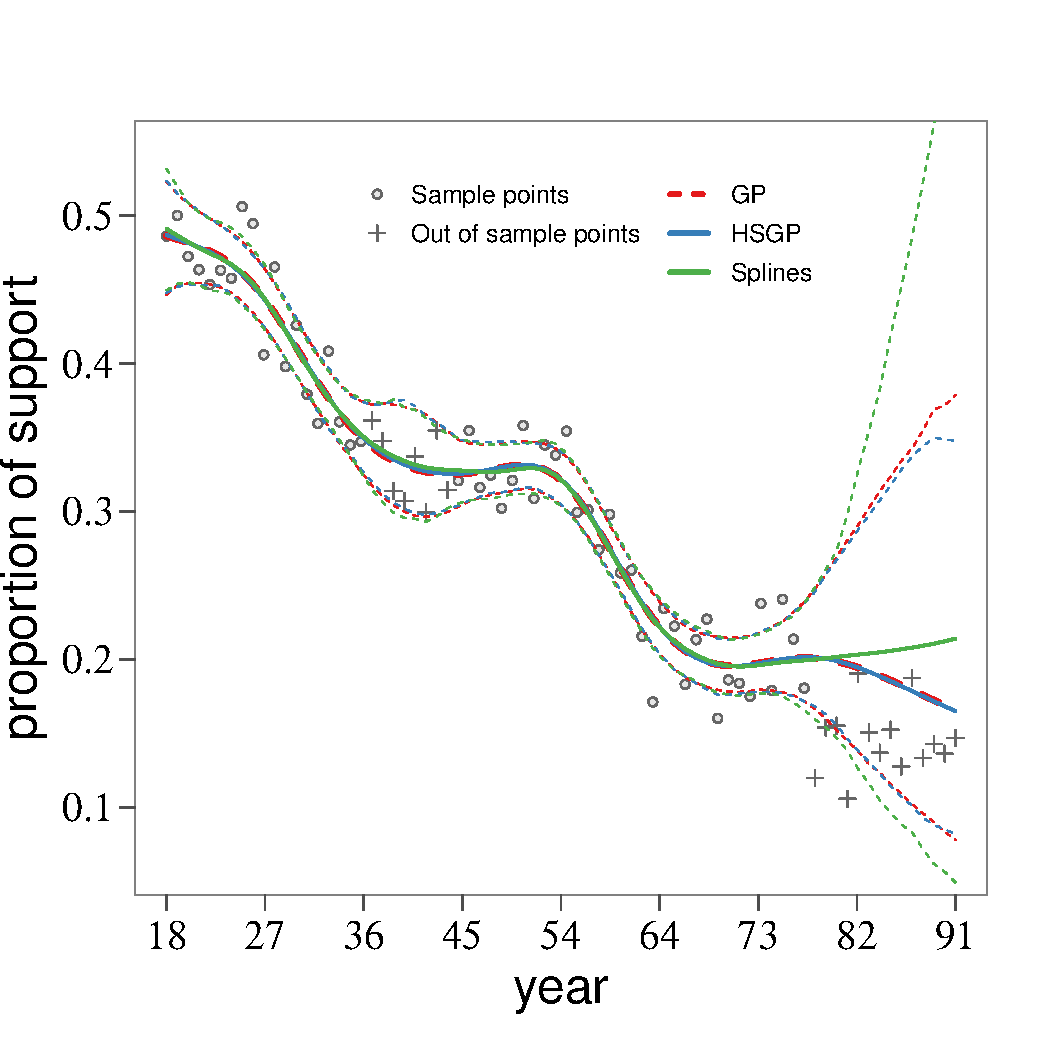
\includegraphics[scale=0.50]{ch5_fig12_Posteriors_gaydata.pdf}
\caption{Posterior mean predictive distributions of the proposed HSGP model, the regular GP model, and the Splines model. 95\% credible intervals are plotted as dashed lines.}
  \label{ch5_fig12_Posteriors_gaydata}
\end{figure}

For the HSGP model, different models with different number of basis functions and boundary factor have been fitted. The root mean square errors (RMSE) for every one of these models have been computed against the regular GP model, and plotted as a function of the number of basis functions $m$ and boundary factor $c$ in Figure \ref{ch5_fig13_MSE_train_BF_gaydata}-left, for sample data, and in Figure \ref{ch5_fig13_MSE_train_BF_gaydata}-right, for test data. As the boundary factor increases, more basis functions are needed for a accurate approximation, as it was expected.

Figure \ref{ch5_fig14_MSE_train_gaydata} shows the RMSE of the regular GP, HSGP and splines models computed against the actual data, for training and test data, as a function of the number of basis functions $m$ and boundary factor $c$ for the HSGP model, and  knots for the splines model. We can see how the splines models do not extrapolate data properly (Figure \ref{ch5_fig14_MSE_train_gaydata}-right). 

Figure \ref{ch5_fig14_1_time_gaydata} shows computational times, in seconds per iteration (iteration of the HMC sampling method), as a function of the number of basis functions $m$, for the HSGP model, and knots, for the splines model. The computational times is represented in the y-axis which is on a logarithmic scale. The HSGP model is on average roughly 15 times faster than the regular GP and 5 times faster than the spline model, for this particular case and univariate input space. Computation time increases relatively slight with the number of basis functions in a univariate input space, as can be seen in the figure.

The Stan model codes for the exact GP, the approximate GP and the splines models of this case study can be found online at {\small \url{https://github.com/gabriuma/basis_functions_approach_to_GP/tree/master/Paper/Case-study_Same-sex-marriage-data}}.

%\begin{lstlisting}[breaklines]
%https://github.com/gabriuma/basis_functions_approach_to_GP/tree/master/Paper/Case-study_Same-sex-marriage-data
%\end{lstlisting}

\begin{figure}
\centering
\subfigure{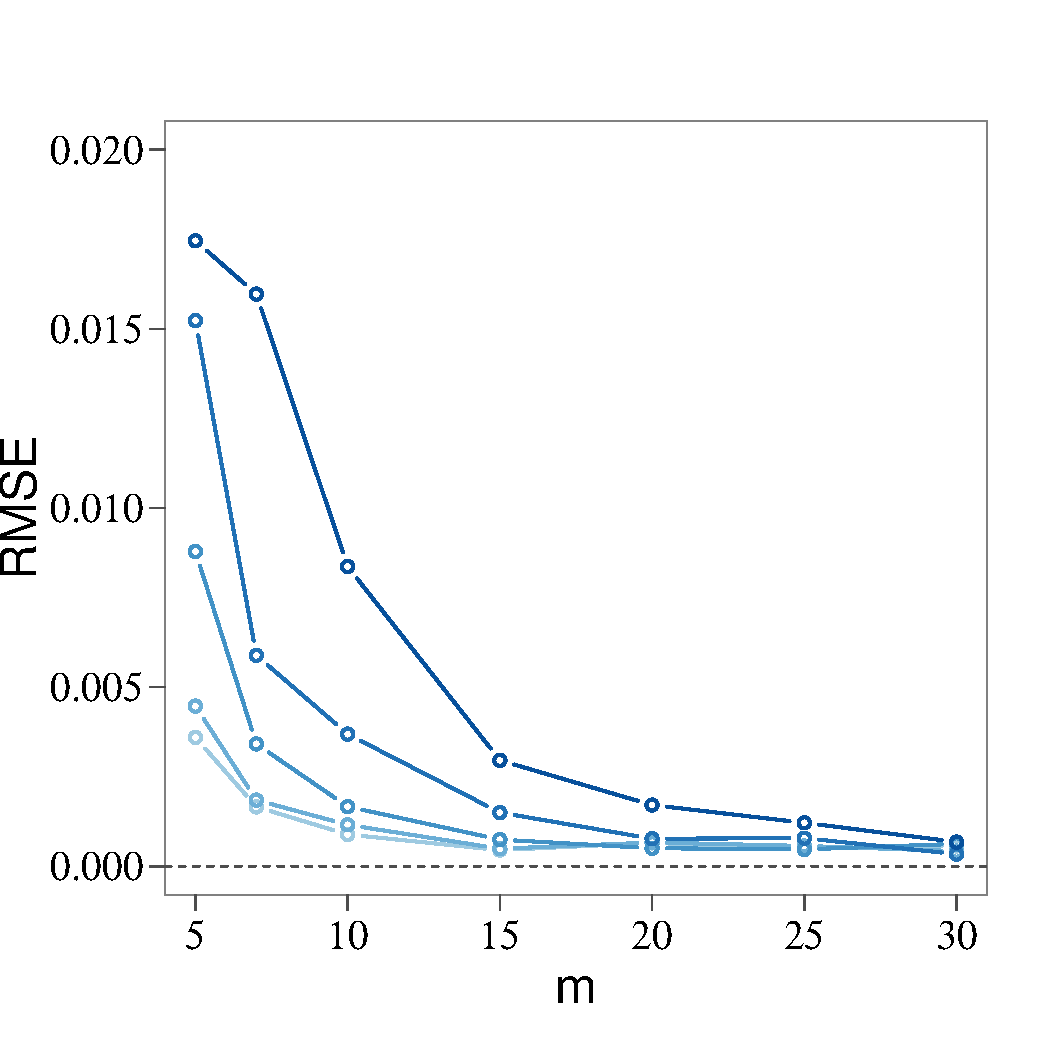
\includegraphics[scale=0.38, trim = 0mm 0mm 5mm 0mm, clip]{ch5_fig13_MSE_train_BF_gaydata.pdf}}
\subfigure{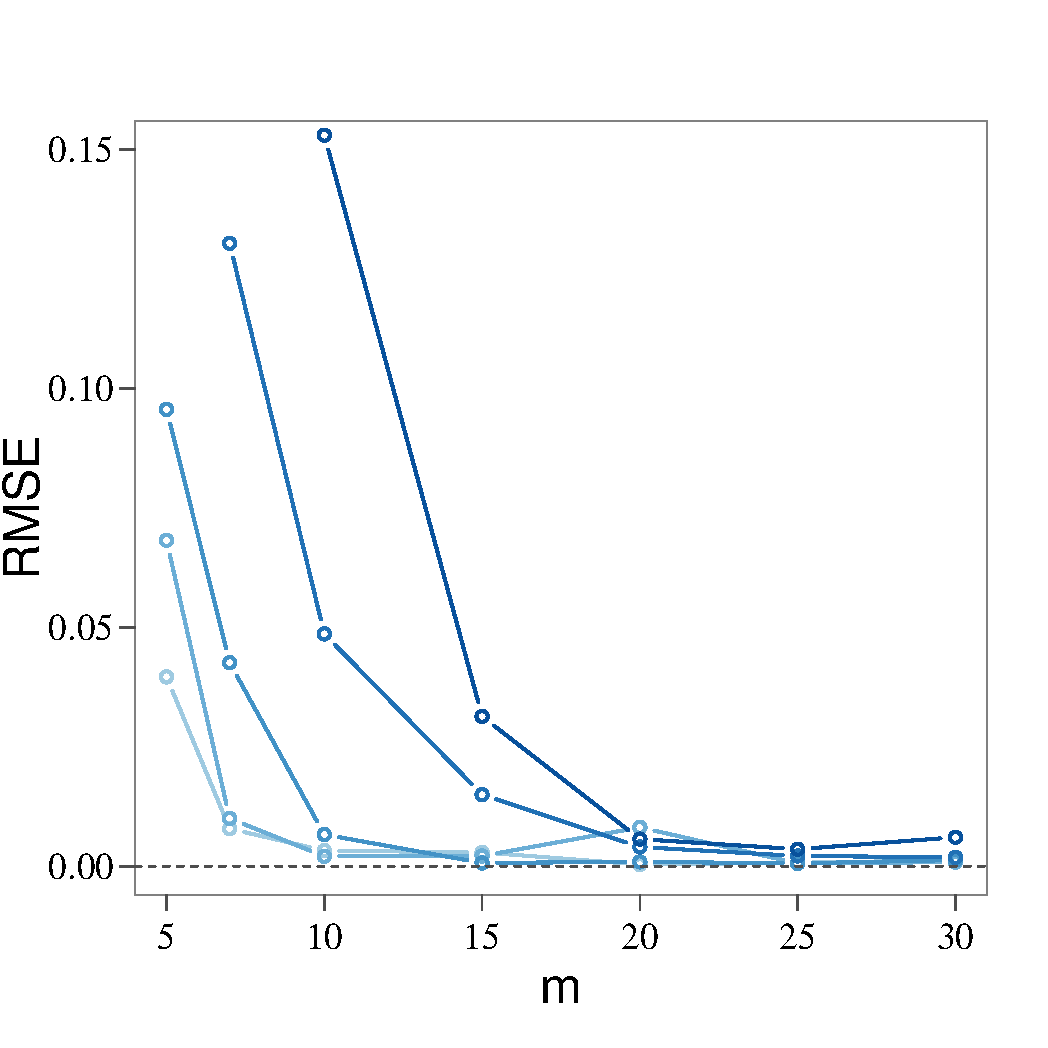
\includegraphics[scale=0.38, trim = 0mm 0mm 10mm 0mm, clip]{ch5_fig13_MSE_pred_BF_gaydata.pdf}}
\subfigure{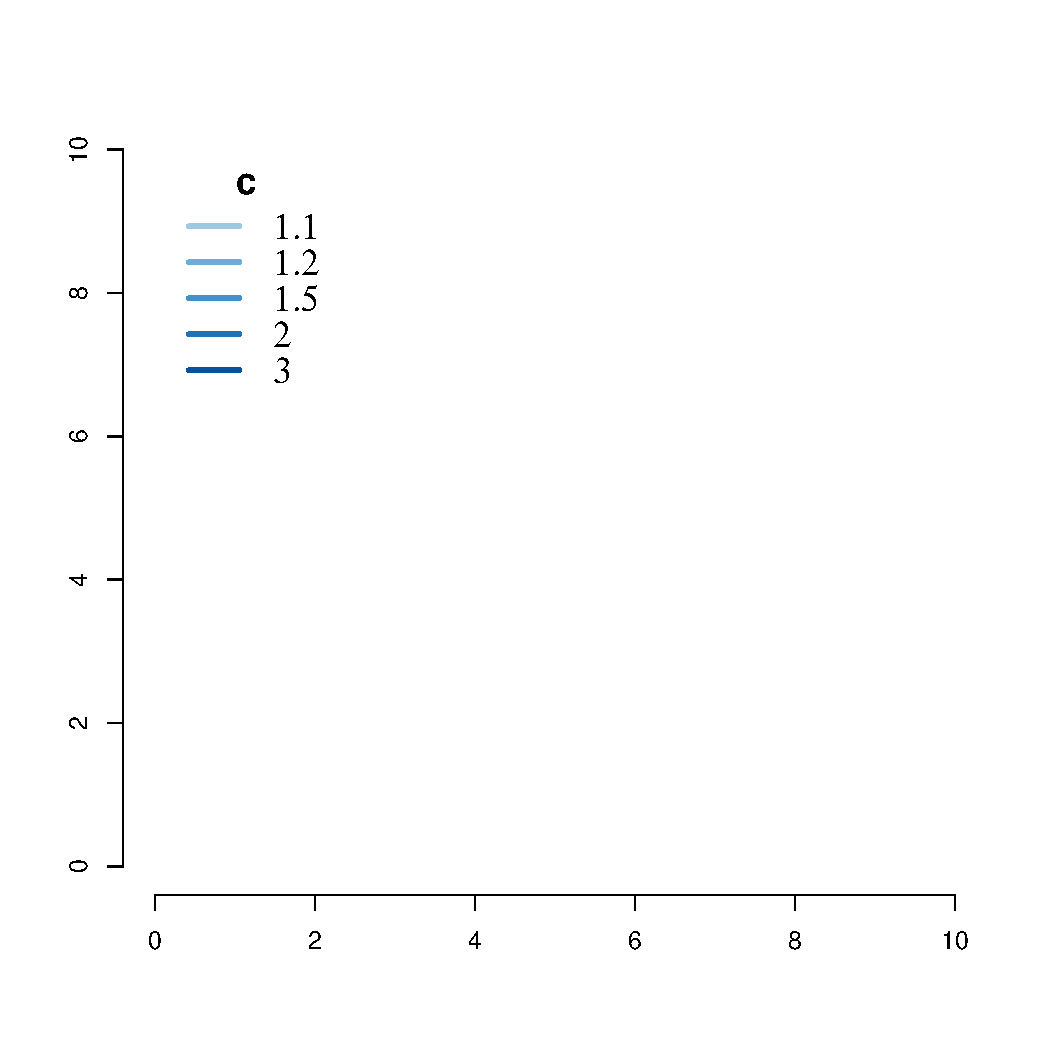
\includegraphics[scale=0.40, trim = 28mm 45mm 119mm 0mm, clip]{ch5_fig13_legend_gaydata.pdf}}
\caption{Root mean square error (RMSE) of the HSGP model, computed against the regular GP model, as a function of the number of basis functions $m$ and boundary factor $c$. RMSE for sample data (left) and RMSE for out-of-sample data (right).}
  \label{ch5_fig13_MSE_train_BF_gaydata}
\end{figure}

\begin{figure}
\centering
\subfigure{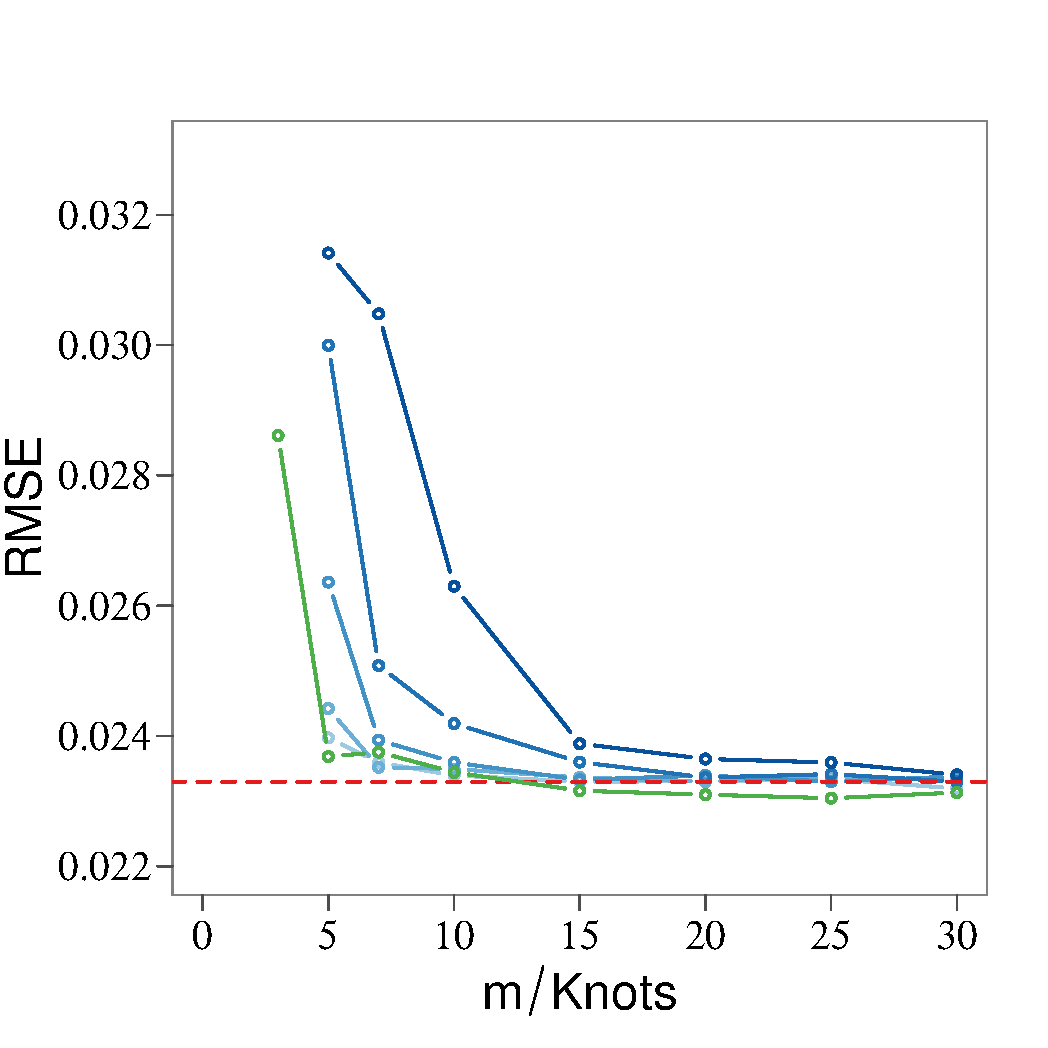
\includegraphics[scale=0.38, trim = 0mm 0mm 5mm 0mm, clip]{ch5_fig14_MSE_train_gaydata.pdf}}
\subfigure{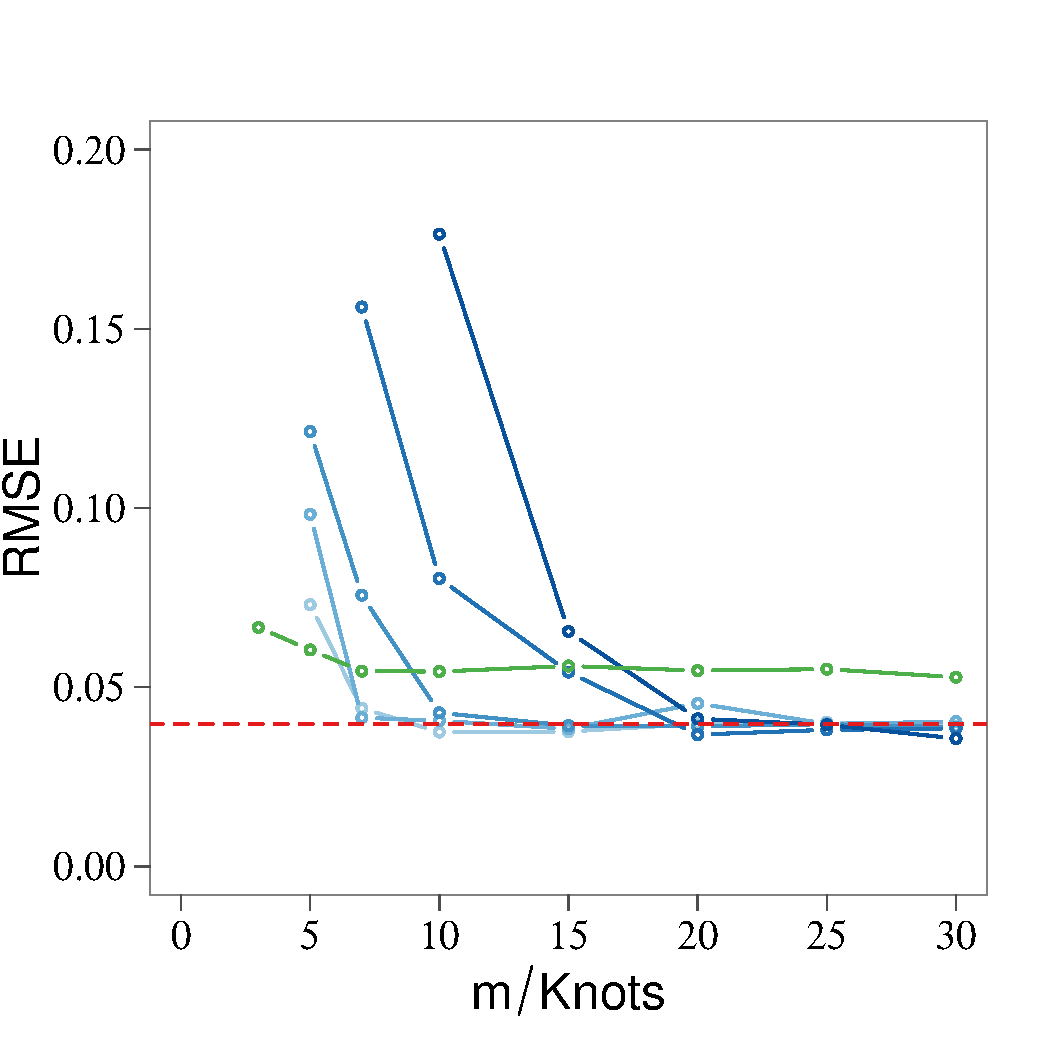
\includegraphics[scale=0.38, trim = 0mm 0mm 10mm 0mm, clip]{ch5_fig14_MSE_pred_gaydata.pdf}}
\subfigure{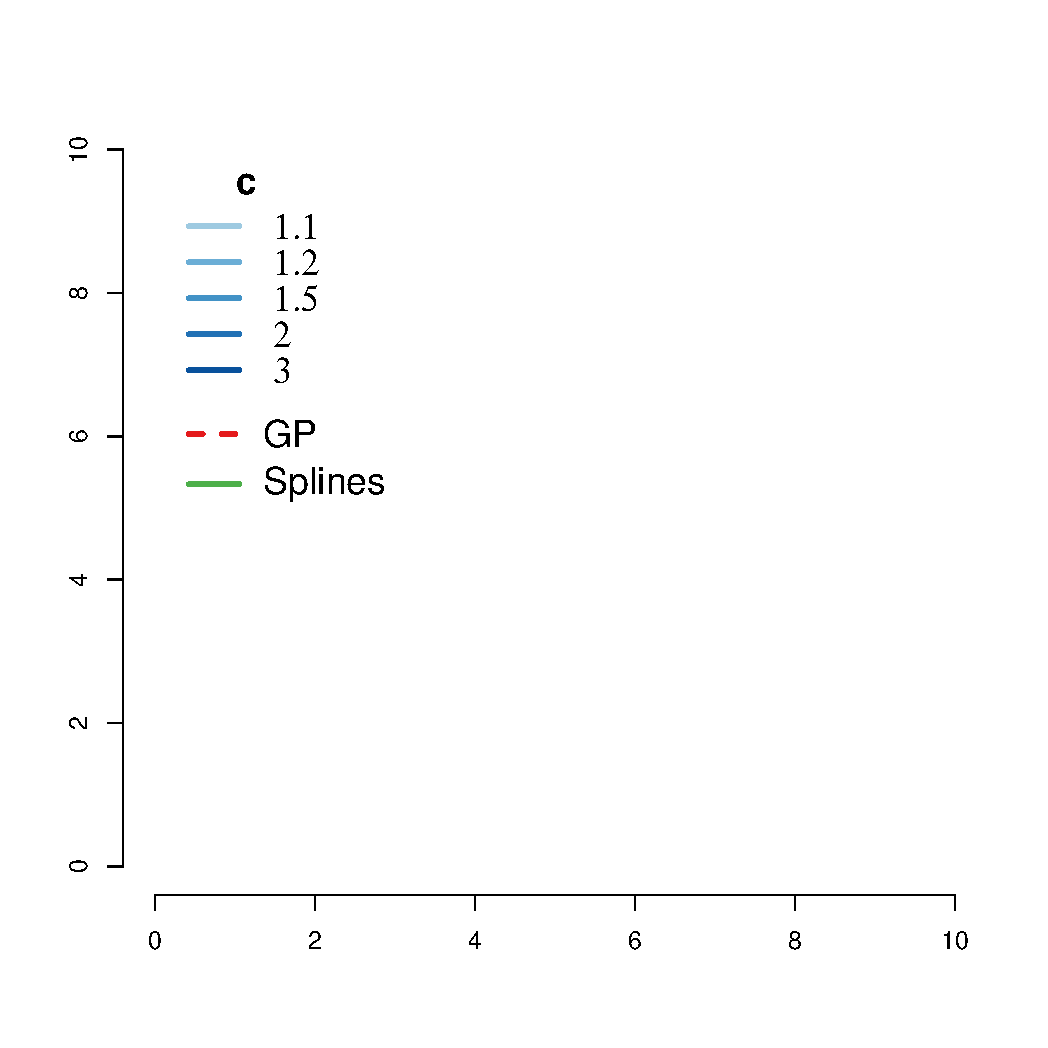
\includegraphics[scale=0.40, trim = 27mm 35mm 112mm 0mm, clip]{ch5_fig14_legend_gaydata.pdf}}
\caption{Root mean square error (RMSE) of the different methods, regular GP, HSGP and splines models, computed against the actual data, as a function of the number of basis functions $m$ and boundary factor $c$ for the HSGP model, and knots for the splines model. RMSE for sample data (left) and RMSE for out-of-sample data (right).}
  \label{ch5_fig14_MSE_train_gaydata}
\end{figure}

\begin{figure}
\centering
\subfigure{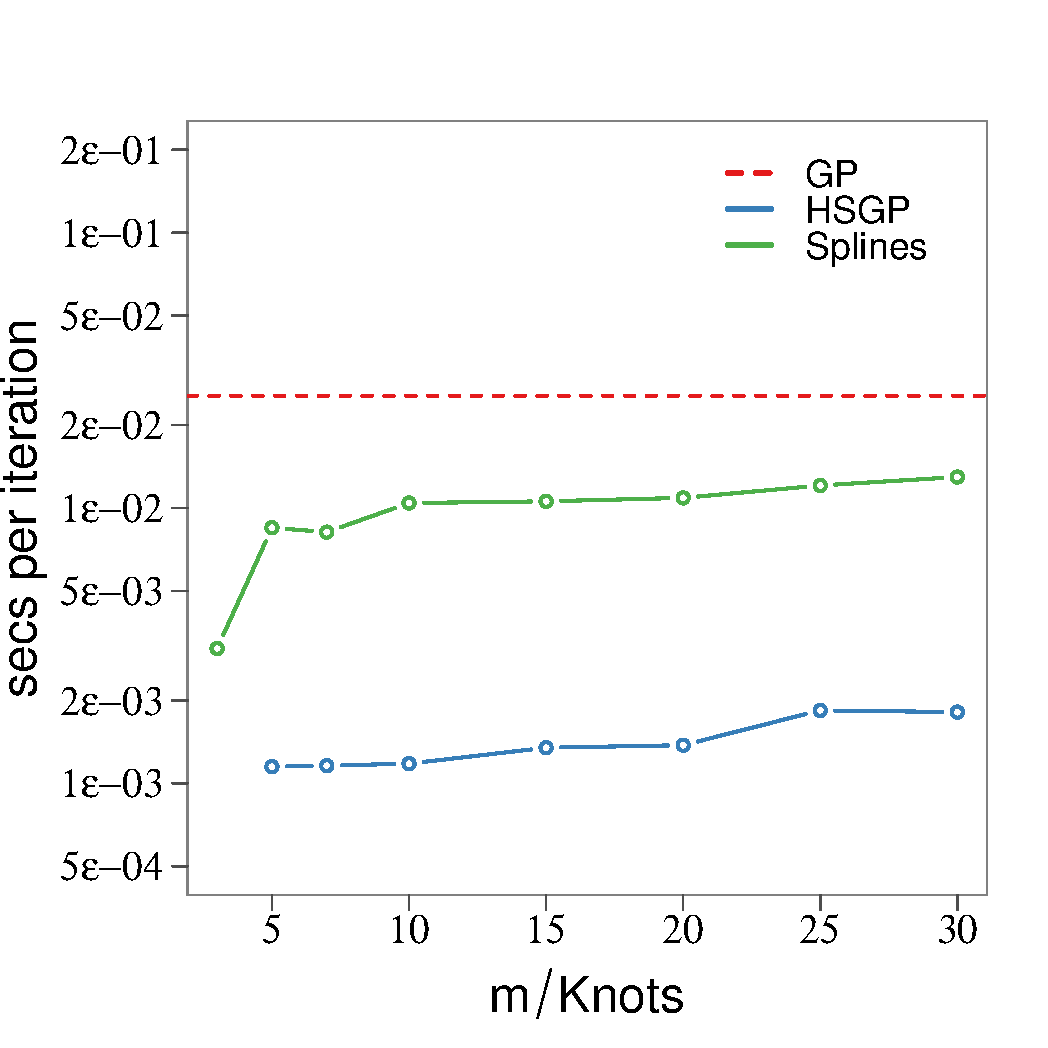
\includegraphics[scale=0.38, trim = 0mm 0mm 10mm 0mm, clip]{ch5_fig14_1_time_gaydata.pdf}}
\caption{Computational time (y-axis), in seconds per iteration (iteration of the HMC sampling method), as a function of the number of basis functions $m$ and knots. The y-axis is in a logarithmic scale.}
  \label{ch5_fig14_1_time_gaydata}
\end{figure}


\section{Case study of simulated data for a bivariate function}

This example consists of a simulated dataset with $n=120$ ($i=1,\dots,n$) single draws from a GP prior as function of input values $\bm{x}_i \in \{[-1,1],[-1,1]\} \subset {\rm I\!R}^2$ in a bivariate input space ($D=2$). A squared exponential covariance function, with hyperparameters marginal variance $\alpha=1$ and lengthscales $\ell_1=0.10$, for the first input dimension, and $\ell_2=0.35$, for the second input dimension, is used for the GP prior. Gaussian noise standard deviation $\sigma=0.2$ was added to the GP draws to form the final noisy set of observations $\bm{y} \in {\rm I\!R}^{120}$.

The regular GP model over the outcome variable $\bm{y}$ can be written as follows,
%
\begin{eqnarray*}\label{ch5_eq_latentgp_simudata2}
\begin{split}
\bm{y} &= \bm{f} + \bm{\epsilon} \\
\bm{\epsilon} &\sim \Normal(0, \sigma^2  I) \\
f(\bm{x}) &\sim \mathcal{GP}(0, k(\bm{x}, \bm{x}', \theta)),
\end{split}
\end{eqnarray*}

\noindent where $\bm{f}=\{f(\bm{x}_i)\}_{i=1}^{120}$ represents the underlying function at the input values $\bm{x_i}\in {\rm I\!R}^{2}$, $\bm{\epsilon}$ is the Gaussian noise term with variance $\sigma^2$, and $I$ represents the identity matrix. The function $f:{\rm I\!R}^2 \to {\rm I\!R}$ is a GP prior with a multivariate squared exponential covariance function $k(\bm{x}_i,\bm{x}_j,\theta)$, which depends on the inputs $\bm{x}$ and hyperparameters $\theta=\{\alpha,\ell_1,\ell_2\}$. The hyperparameters $\alpha$, $\ell_1$ and $\ell_2$ represent the marginal variance and lengthscales for first and second input dimensions, respectively, of the GP process. Saying that the function $f(\cdot)$ follows a GP model is equivalent to say that $\bm{f}$ is multivariate Gaussian distributed with covariance matrix $\bm{K}$, where $K_{ij}=k(\bm{x}_i,\bm{x}_j,\theta)$, with $i,j=1,\dots,120$.

The marginalized form, by integrating out the latent values $\bm{f}$, of the previous latent GP model results:
%
\begin{equation*}\label{ch5_eq_marginalizedgp_simudata2}
\bm{y} \sim \Normal(0, \bm{K} + \sigma^2 I ).
\end{equation*}

In the HSGP model with $2$ input dimensions, the latent function $f(\bm{x})$ is approximated as in equation (12)% (\ref{eq_approxf_multi})
, with the $2$-dimensional squared exponential spectral density $S$ as in equation (1)% (\ref{eq_specdens_inf})
, and the $2$-vector of eigenvalues $\bm{\lambda}_j$ and the multivariate eigenfunctions $\phi_j$ as in equations (9) %(\ref{eq_eigenfunction_multi})
 and (10)% (\ref{eq_eigenvalue_multi})
 , respectively.


In order to do model comparison, in addition to the regular GP and HSGP models, a two-dimensional splines-based model is also fitted using a cubic spline basis, penalized by the conventional integrated square second derivative cubic spline penalty \citep{wood2017generalized}, and implemented in the R-package \textit{mgcv} \citep{wood2011mgcv}. A Bayesian approach is used to fit this spline model using the R-package \textit{brms} \citep{burkner2017brms}.

Figure \ref{ch5_fig15_Posteriors_exII} shows the data-generating GP function, from where the dataset was drawn, and the mean posterior predictive functions of the three models, the regular GP, the HSGP, and the splines, fitted over the dataset. Sample observations are also plotted as circles. For the HSGP model, $m_1=40$ and $m_2=40$ basis functions for each dimension respectively, were used, which lead to a total of 1600 multivariate basis functions. A boundary factor for each dimension $c_1=1.5$ and $c_2=1.5$ were used. For the splines model, 40 knots in each dimension were used.

Figure \ref{ch5_fig16_errors_exII} shows the difference functions between the data-generating function and the GP, HSGP and splines models, respectively.

\begin{figure}
\begin{center}
\begin{tabular}{ c c c}
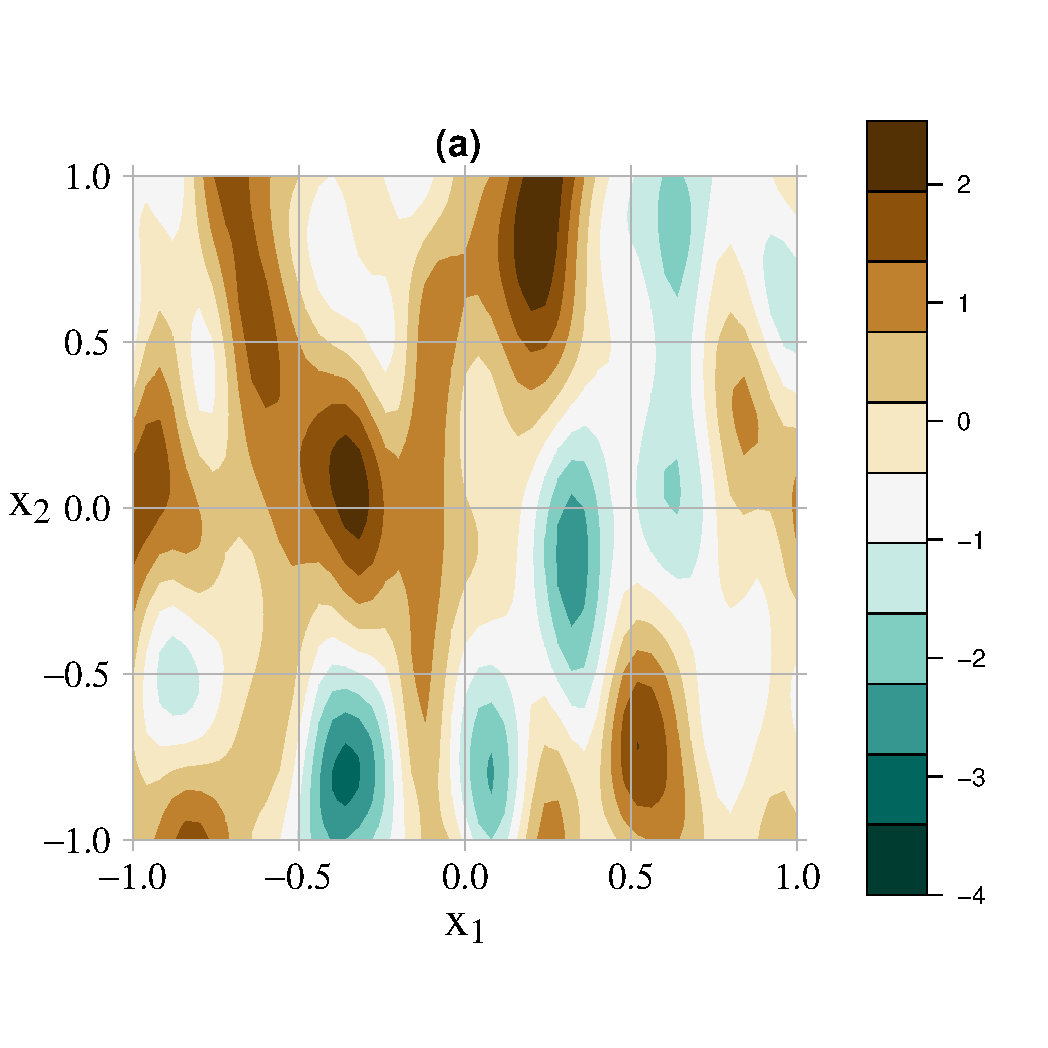
\includegraphics[scale=0.40, trim = 0mm 33mm 35mm 20mm, clip]{ch5_fig15_truefun_exII.pdf} & \hspace{-5mm} 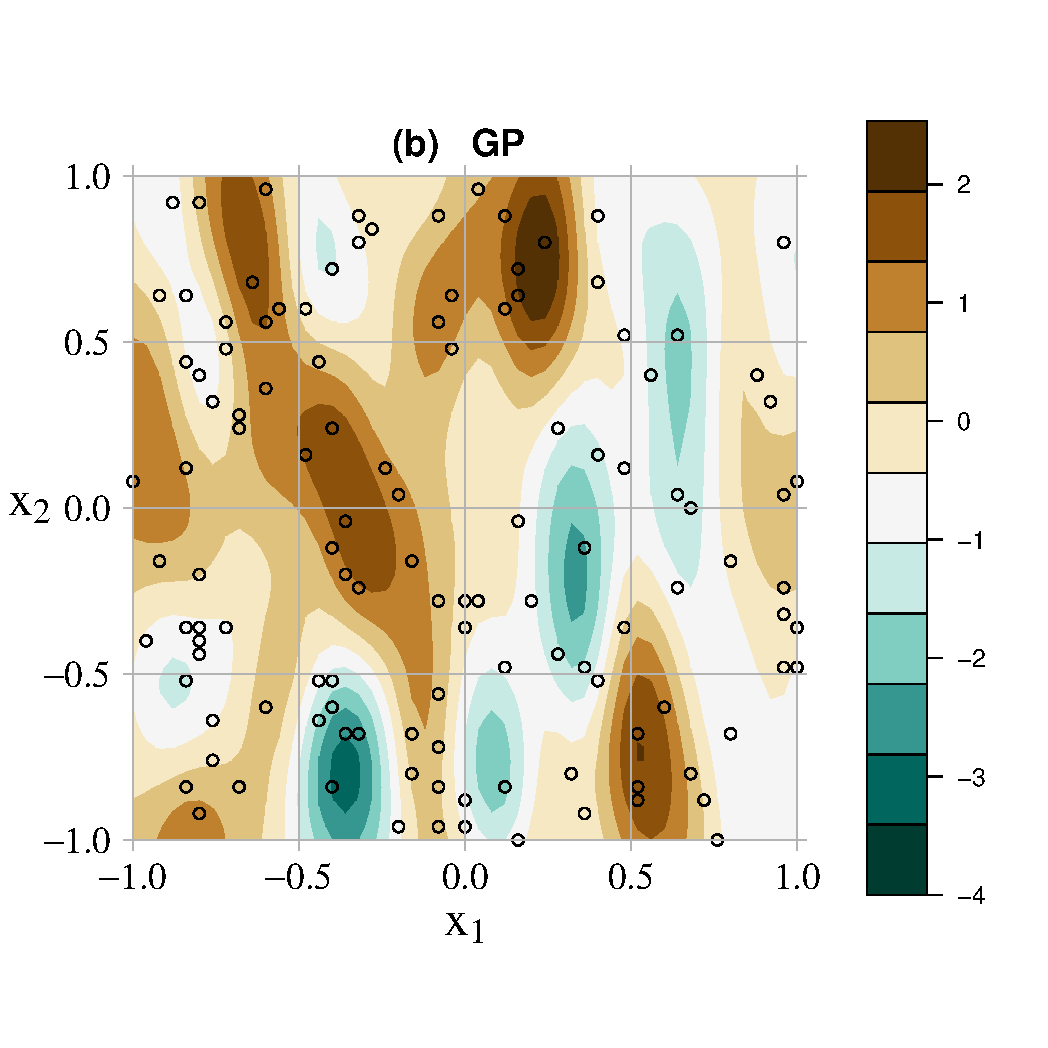
\includegraphics[scale=0.40, trim = 19mm 33mm 35mm 20mm, clip]{ch5_fig15_gpfun_exII.pdf} & \hspace{-5mm}\multirow{-5.5}{*}{ 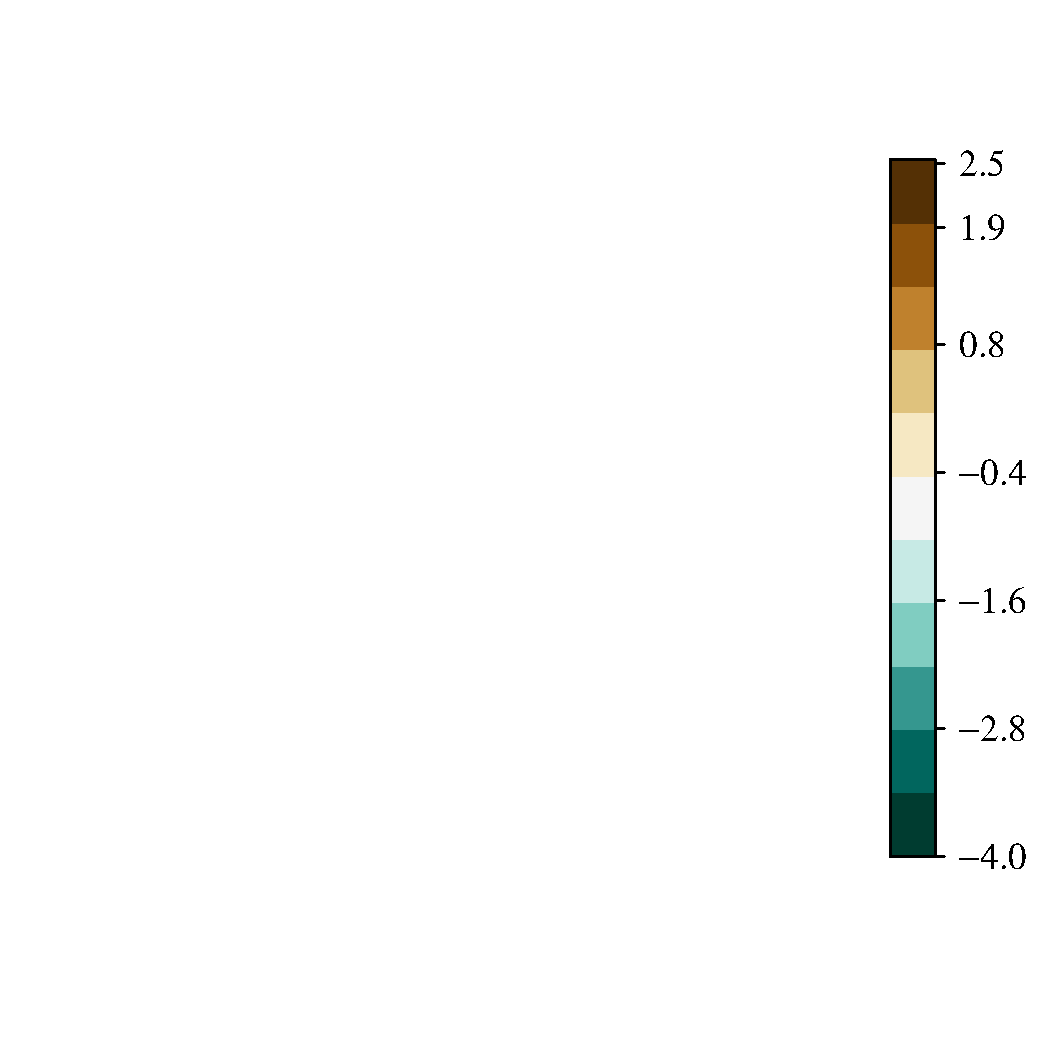
\includegraphics[scale=0.35, trim = 150mm 18mm 0mm 10mm, clip]{ch5_fig15_colorbar_vertical_exII.pdf}}\\ 
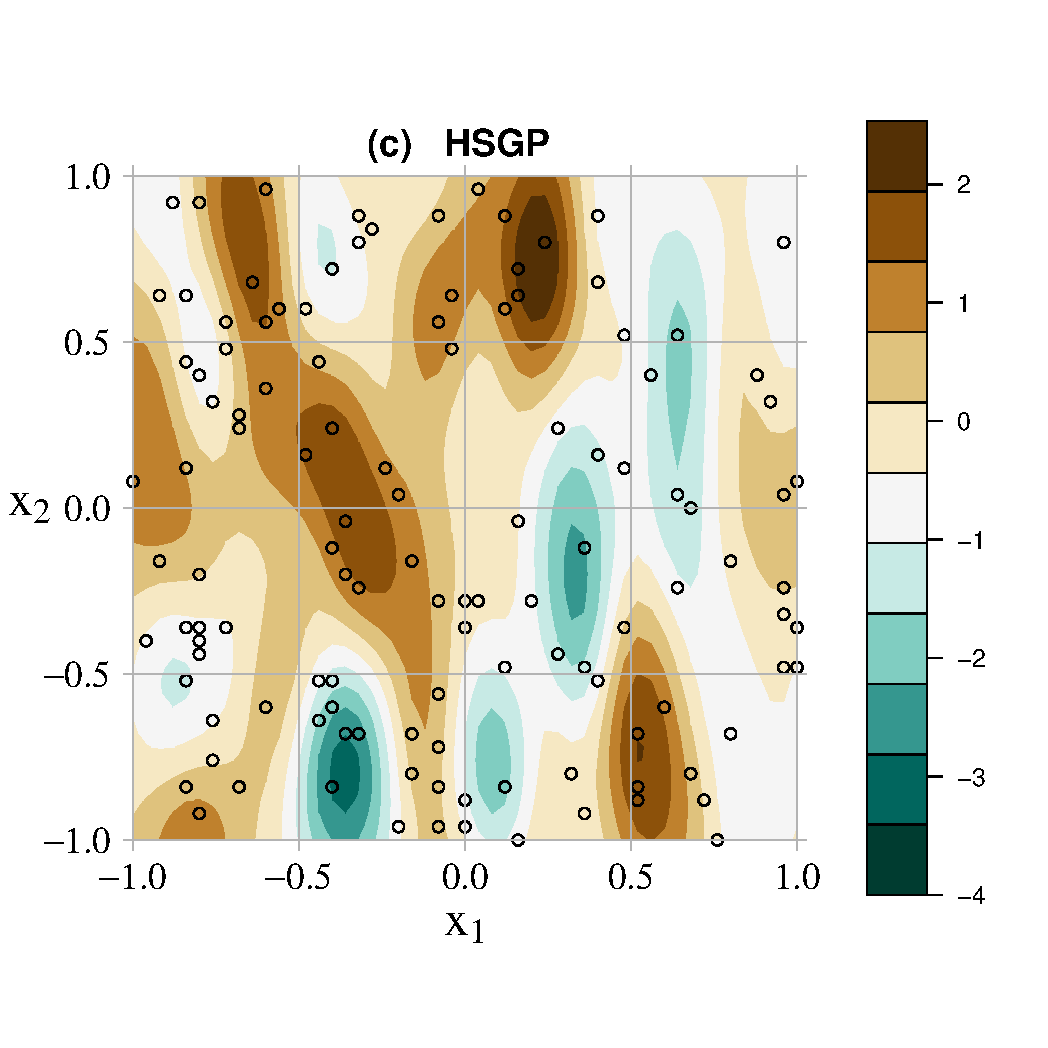
\includegraphics[scale=0.40, trim = 0mm 18mm 35mm 20mm, clip]{ch5_fig15_bffun_exII.pdf}  & \hspace{-5mm} 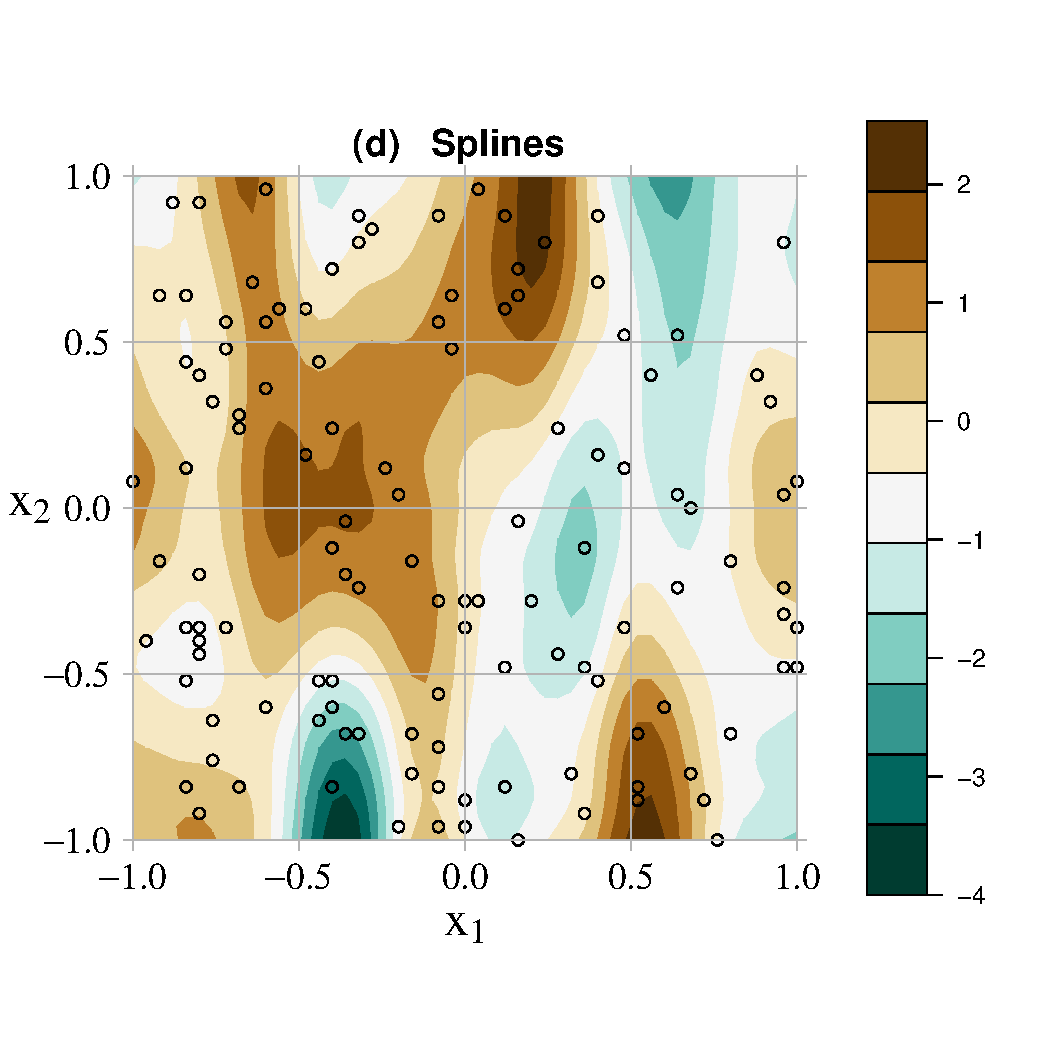
\includegraphics[scale=0.40, trim = 19mm 18mm 35mm 20mm, clip]{ch5_fig15_spfun_exII.pdf}
\end{tabular}
\end{center}
\caption{(a) Data-generating function. (b) Mean posterior predictive function of the GP model. (c) Mean posterior predictive function of the HSGP model. (d) Mean posterior predictive function of the splines model. Sample points are plotted as circles}
  \label{ch5_fig15_Posteriors_exII}
\end{figure}


\begin{figure}
\centering
\subfigure{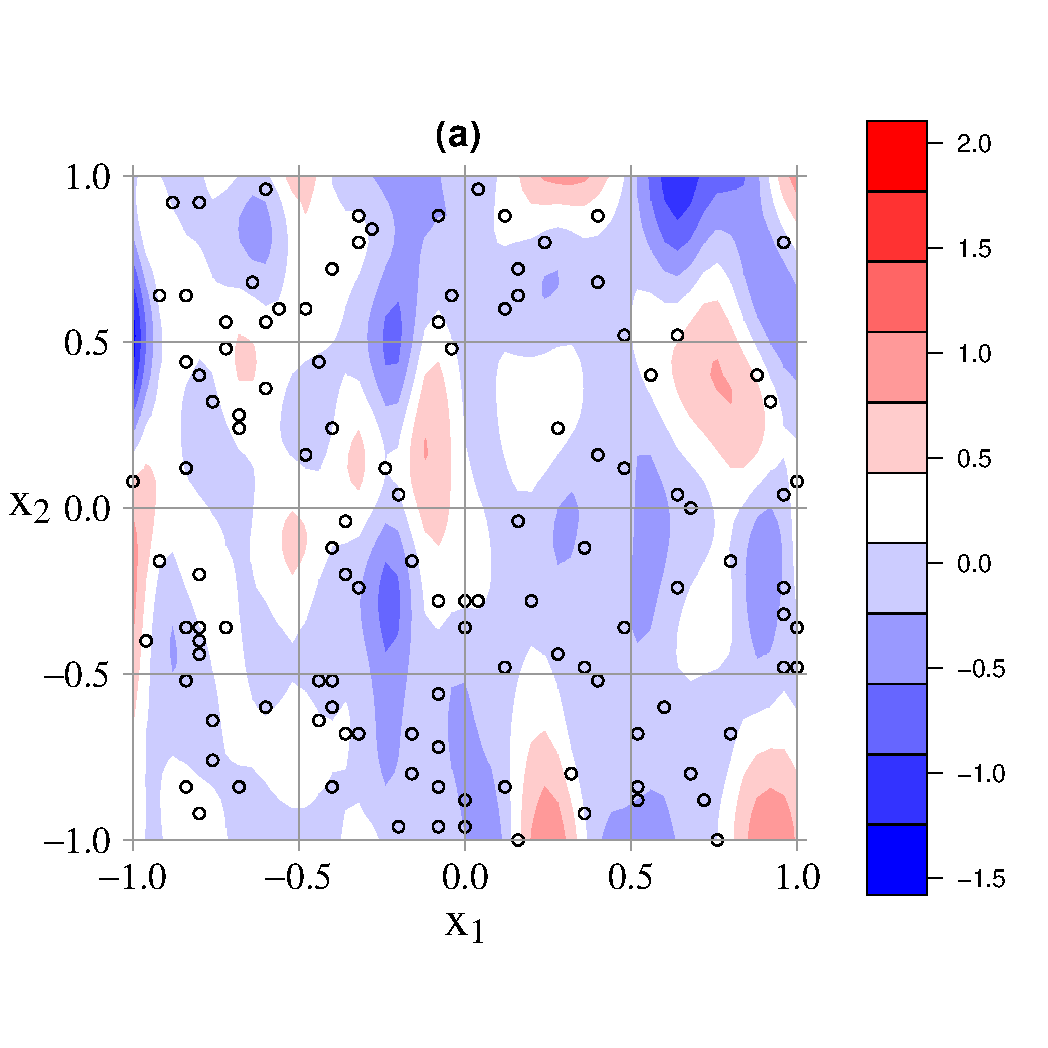
\includegraphics[scale=0.36, trim = 1mm 18mm 39.2mm 20mm, clip]{ch5_fig16_errorGP_exII.pdf}}
\subfigure{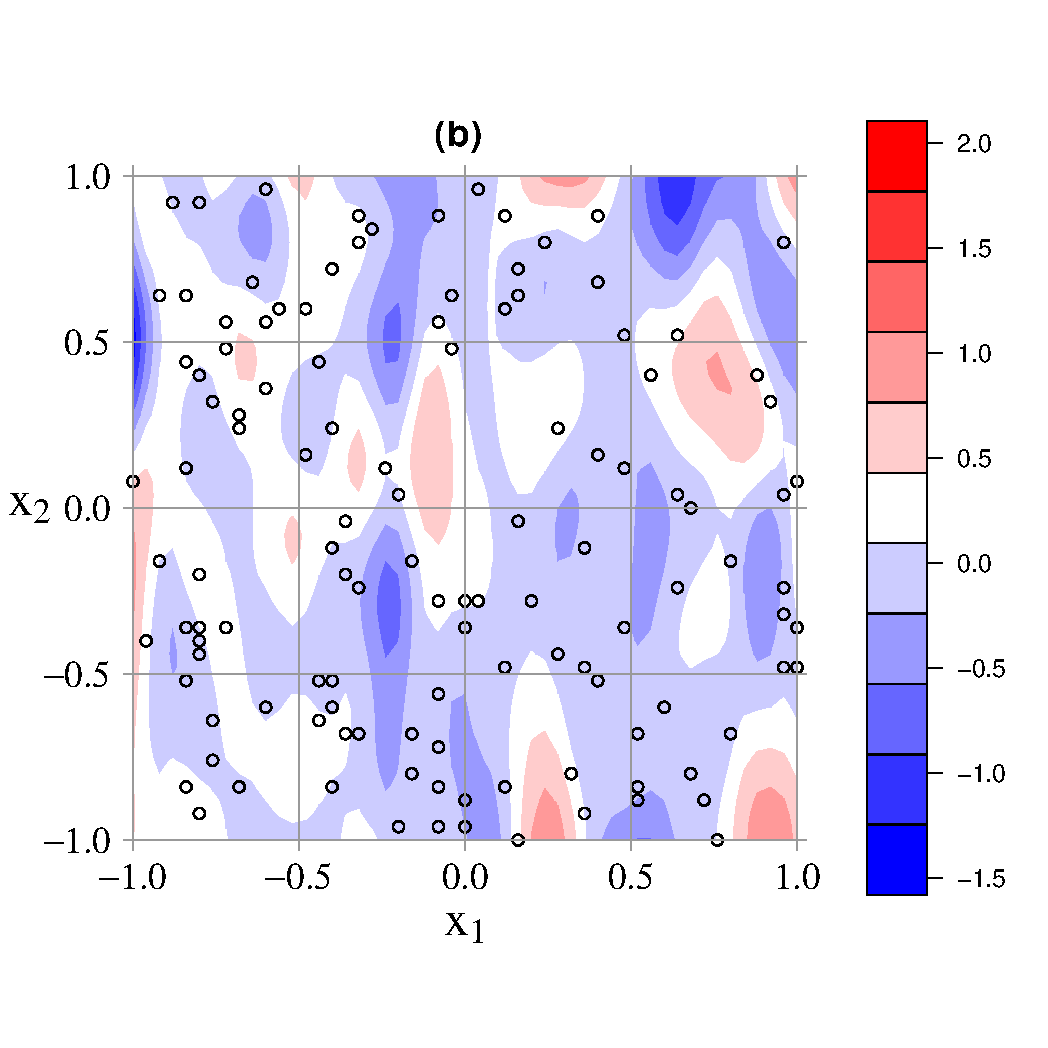
\includegraphics[scale=0.36, trim = 19mm 18mm 39.2mm 20mm, clip]{ch5_fig16_errorHSGP_exII.pdf}}
\subfigure{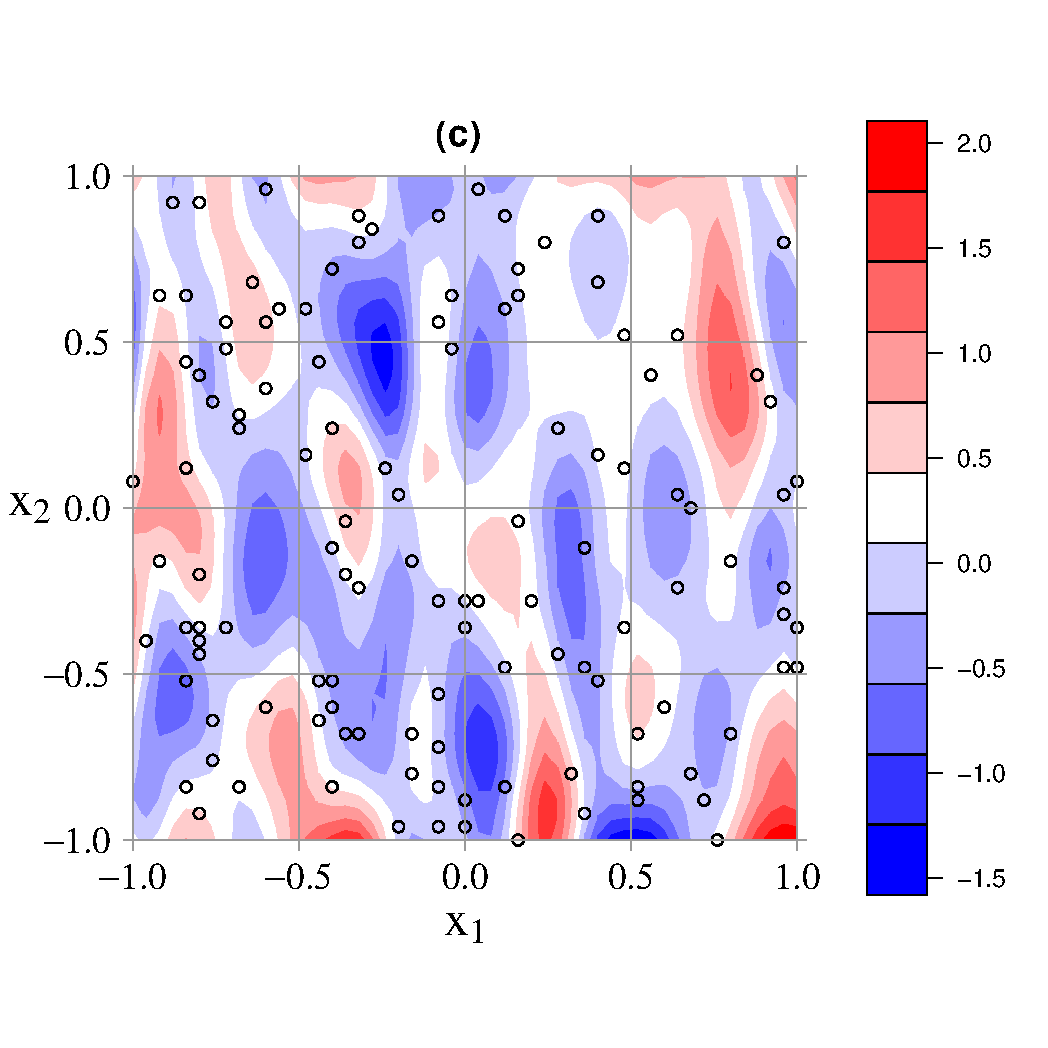
\includegraphics[scale=0.36, trim = 19mm 18mm 39.2mm 20mm, clip]{ch5_fig16_errorSP_exII.pdf}}
\subfigure{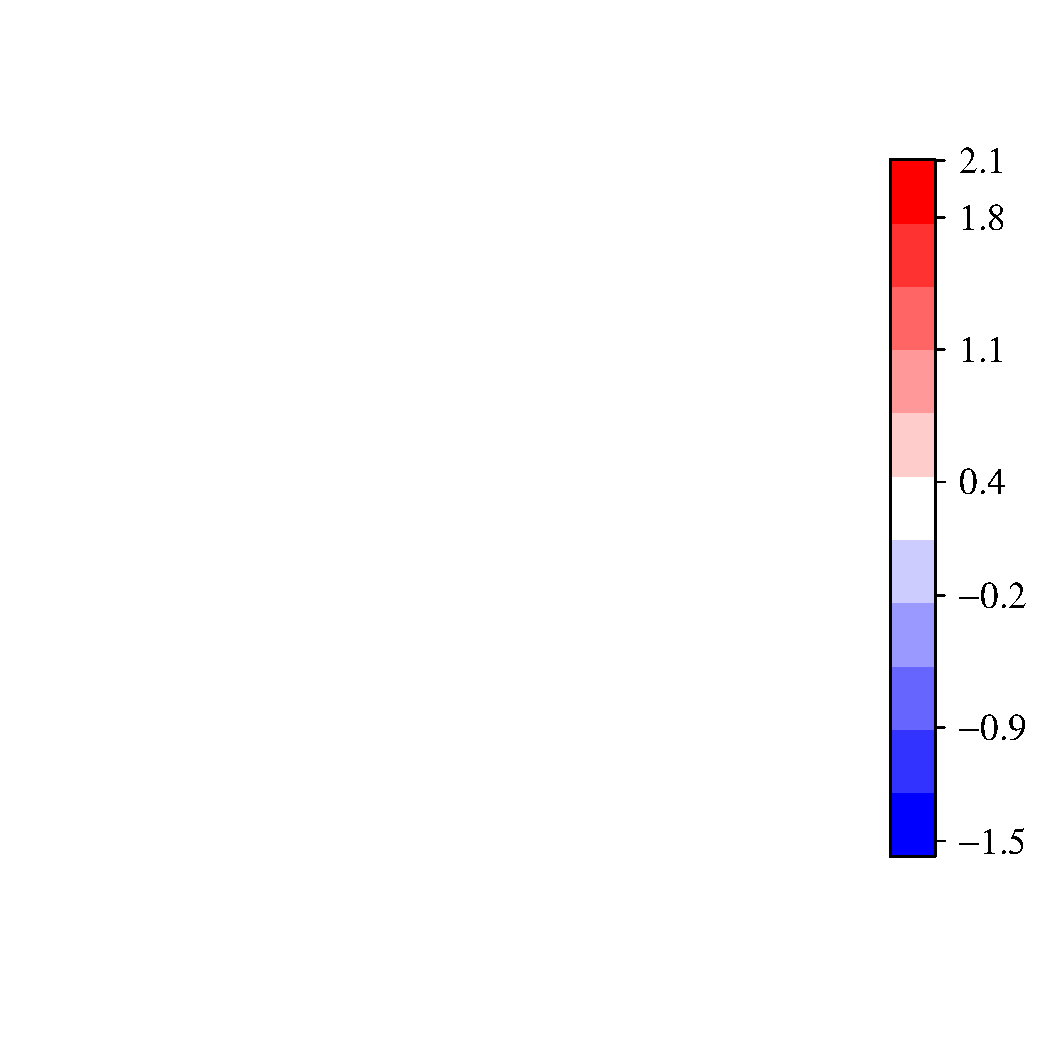
\includegraphics[scale=0.30, trim = 150mm 5mm 0mm 20mm, clip]{ch5_fig16_error_colorbar_exII.pdf}}
\caption{Mean error between the data-generating function and the GP (a), HSGP (b) and splines (c) models. Sample points are plotted as circles.}
  \label{ch5_fig16_errors_exII}
\end{figure}

In order to assess performance of the models as a function of the number of basis functions and knots, different models with different number of basis functions, for the HSGP model, and different number of knots, for the splines model, have been fitted. In all models, the same number of basis functions and knots per dimension were used. Figure \ref{ch5_fig17_RMSE_exII}-left shows the root mean squared error (RMSE), computed against the data-generating function, as a function of the boundary factor $c$, and the number of univariate basis functions $m$, for the HSGP model, and knots, for the splines model. From Figures \ref{ch5_fig16_errors_exII} and \ref{ch5_fig17_RMSE_exII}-left, it can be seen a close approximation of the HSGP model to the regular GP model. However, the performance of the splines model is significantly worse. 

Figure \ref{ch5_fig17_RMSE_exII}-right shows the computational times of the different models as a function of the boundary factor, number of basis functions and knots. Figure \ref{ch5_fig17_RMSE_exII} reveals that choosing the optimal boundary factor allows for less number of basis functions and less computation time. Even though in a bivariate input space the computation demand increases significantly with the number of dimensions or knots, either the HSGP or spline models work significantly better than regular GP, even for highly wiggly functions that require a high number of basis functions or knots for a accurate approximation. However, serious difficulties with cumputation time were encountered in building the spline model with $50$ knots for this bivariate function.

The Stan model codes for the exact GP, the approximate GP and the splines models of this case study can be found online at {\small \url{https://github.com/gabriuma/basis_functions_approach_to_GP/tree/master/Paper/Case-study_2D-Simulated-data}}.


\begin{figure}
\centering
\subfigure{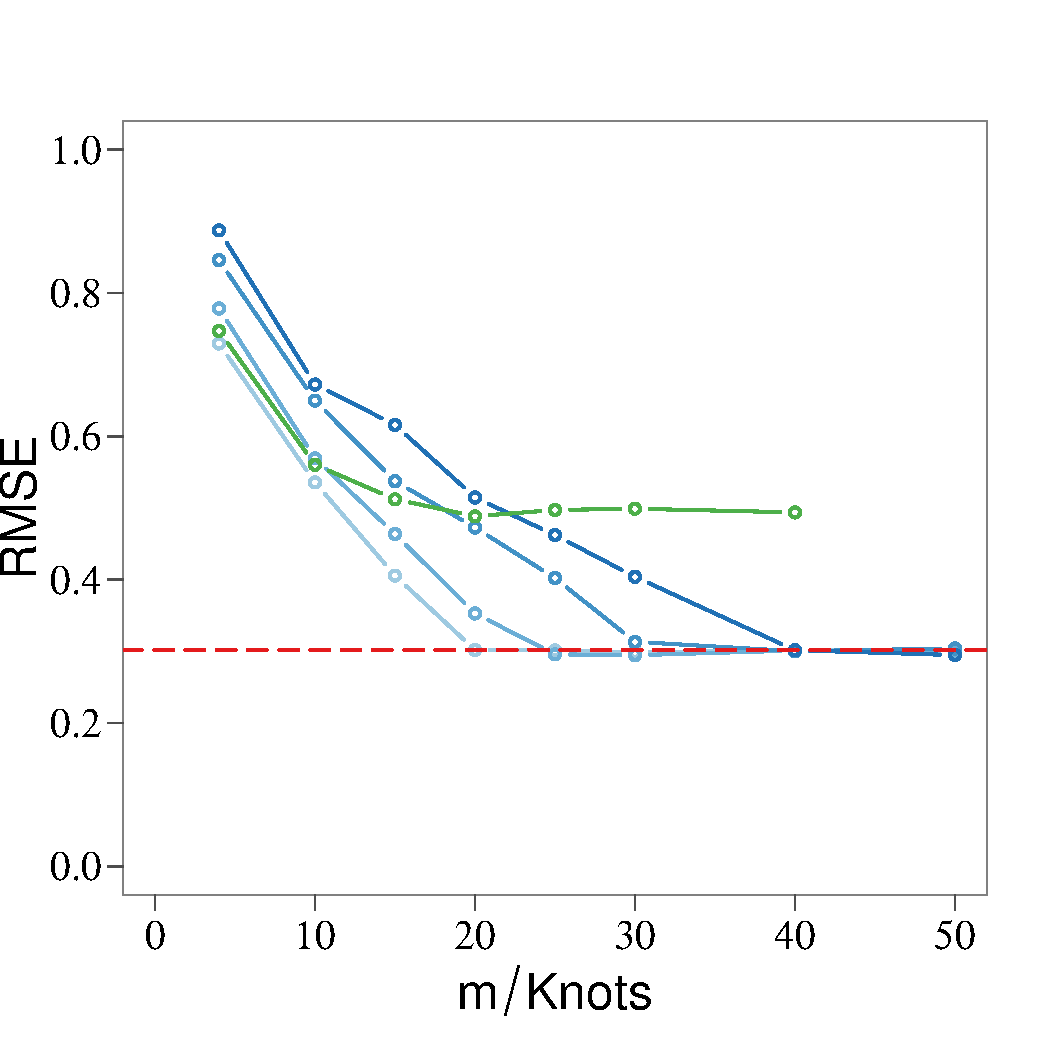
\includegraphics[scale=0.38, trim = 0mm 0mm 5mm 0mm, clip]{ch5_fig17_RMSE_exII.pdf}}
\subfigure{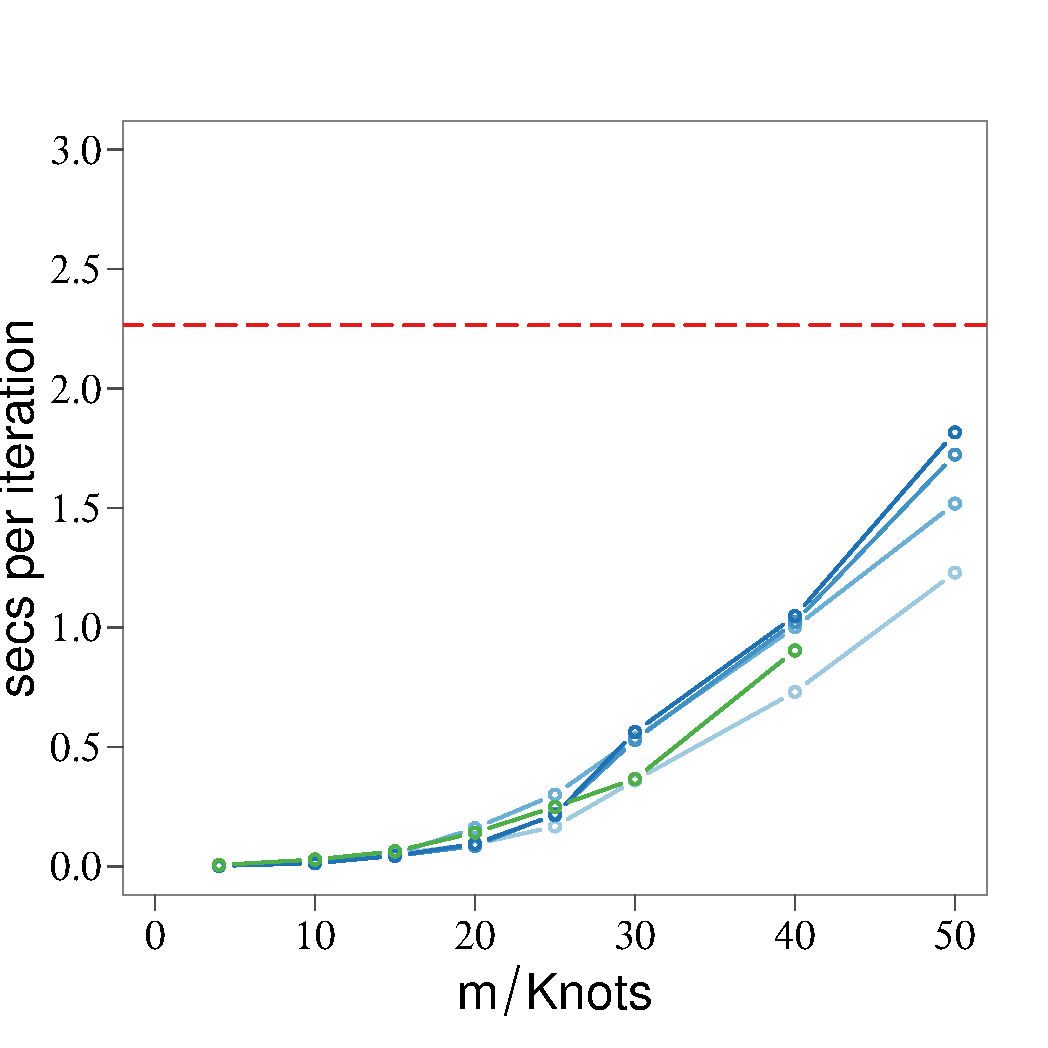
\includegraphics[scale=0.38, trim = 0mm 0mm 10mm 0mm, clip]{ch5_fig17_time_exII.pdf}}
\subfigure{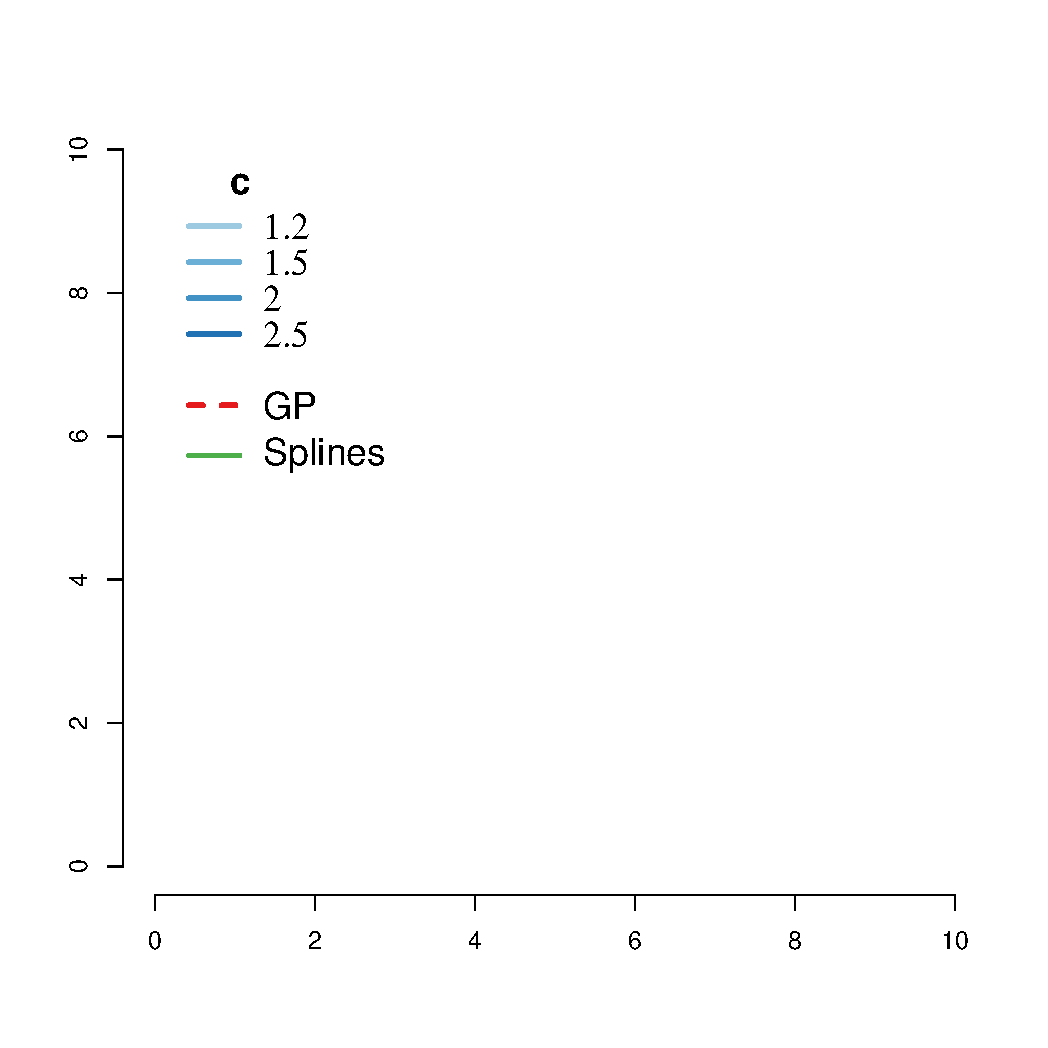
\includegraphics[scale=0.40, trim = 28mm 35mm 112mm 0mm, clip]{ch5_fig17_legend_exII.pdf}}
\caption{Root mean square error (RMSE) (left) and computational time (right) in seconds per iteration (iteration of the HMC sampling method) of the different methods computed against the data-generating function, as a function of the boundary factor $c$, number of basis functions $m$ and knots.}
  \label{ch5_fig17_RMSE_exII}
\end{figure}


\section{Diabetes case study}\label{ch5_sec_bf_caseV}
The next example presents an epidemiological study of diabetes disease. The study aims to relate the probability of suffering from diabetes to some risk factors. The data contains $n=392$ individuals ($i=1,\dots,n$) from which the binary variable of suffering ($y_i=1$) or not suffering ($y_i=0$) from diabetes have been observed. The input vector $\bm{x}_i=(x_{i1},x_{i2},x_{i3},x_{i4}) \in {\rm I\!R}^{4}$, in a 4D input space ($D=4$), contains the risk factors, \textit{Glucose} ($x_{i1}$), \textit{Pregnancy} ($x_{i2}$), \textit{Age} ($x_{i3}$) and \textit{BMI} ($x_{i4}$), per individual $i$. The observational model is a Bernoulli model with parameter the probability $p_i$ of suffering from diabetes per observation $i$,
%
\begin{equation*}
y_i \sim \mathrm{Bernoulli}(p_i).
\end{equation*}

\noindent The goal is to estimate the probability $p_i$ as a function of the risk factors, which function $f(\cdot):{\rm I\!R}^{4} \to {\rm I\!R}$ is modeled as a GP with a multivariate squared exponential covariance function $k$ depending on the risk factors $\bm{x}$ and hyperparameters $\theta=\{\alpha,\ell\}$, and related to the probabilities $p_i$ through the {\it logit} link function,
%
\begin{align*} \label{ch5_eq_gpprior_gay}
p_i &= \mathrm{logit}(f(\bm{x}_i)) \nonumber \\
f(\bm{x}) &\sim \mathcal{GP}(0, k(\bm{x},\bm{x}', \theta).
\end{align*}

\noindent Saying that the function $f(\cdot)$ follows a GP model is equivalent to say that $\bm{f}=\{f(\bm{x}_i)\}_{i=1}^n$ are multivariate Gaussian distributed with covariance matrix $\bm{K}$, where $K_{ij}=k(x_i,x_j,\theta)$, with $i,j=1,\dots,n$. The hyperparameters $\alpha$ and $\ell$ represent the marginal variance and lengthscale, respectively, of the GP process. A scalar lengthscale has been considered in the multivariate covariance function $k$.

In the HSGP model with $D$ input dimensions, the function $f(\bm{x})$ evaluated at input vector $\bm{x} \in {\rm I\!R}^D$ is approximated as in equation (12)% (\ref{eq_approxf_multi})
, with the $D$-dimensional (with a scalar lengthscale) squared exponential spectral density $S$ as in equation (1) %(\ref{eq_specdens_inf}) 
and the $D$-vector of eigenvalues $\bm{\lambda}_j$ and the multivariate eigenfunctions $\phi_j$ as in equations (9) % (\ref{eq_eigenvalue_multi}) 
and (10)% (\ref{eq_eigenfunction_multi})
, respectively.


In order to do model comparison, in addition to the regular GP and HSGP models, a $D$-dimensional spline-based model is also fitted using a cubic spline basis penalized by the conventional integrated square second derivative cubic spline penalty \citep{wood2017generalized} and implemented in the R-package \textit{mgcv} \citep{wood2011mgcv}. A Bayesian approach is used to fit this spline model using the R-package \textit{brms} \citep{burkner2017brms}.

Figure \ref{ch5_fig18_gpfun_diabetes} shows the mean posterior predictions of probabilities ($p_i$) of the three models, the regular GP, the HSGP and the spline, fitted over the dataset with the 2 input dimensions \textit{Glucose} and \textit{Pregnancy} ($D=2$). The binary observations $y_i$ are also plotted in the plots as colored points. For the HSGP model, $m_1=20$ and $m_2=20$ basis functions for each dimension, respectively, were used, which lead to a total of 400 multivariate basis functions. A boundary factor for each dimension $c_1=4$ and $c_2=4$ were used. For the spline model, 20 knots per dimension were used.
%
\begin{figure}
\centering
\subfigure{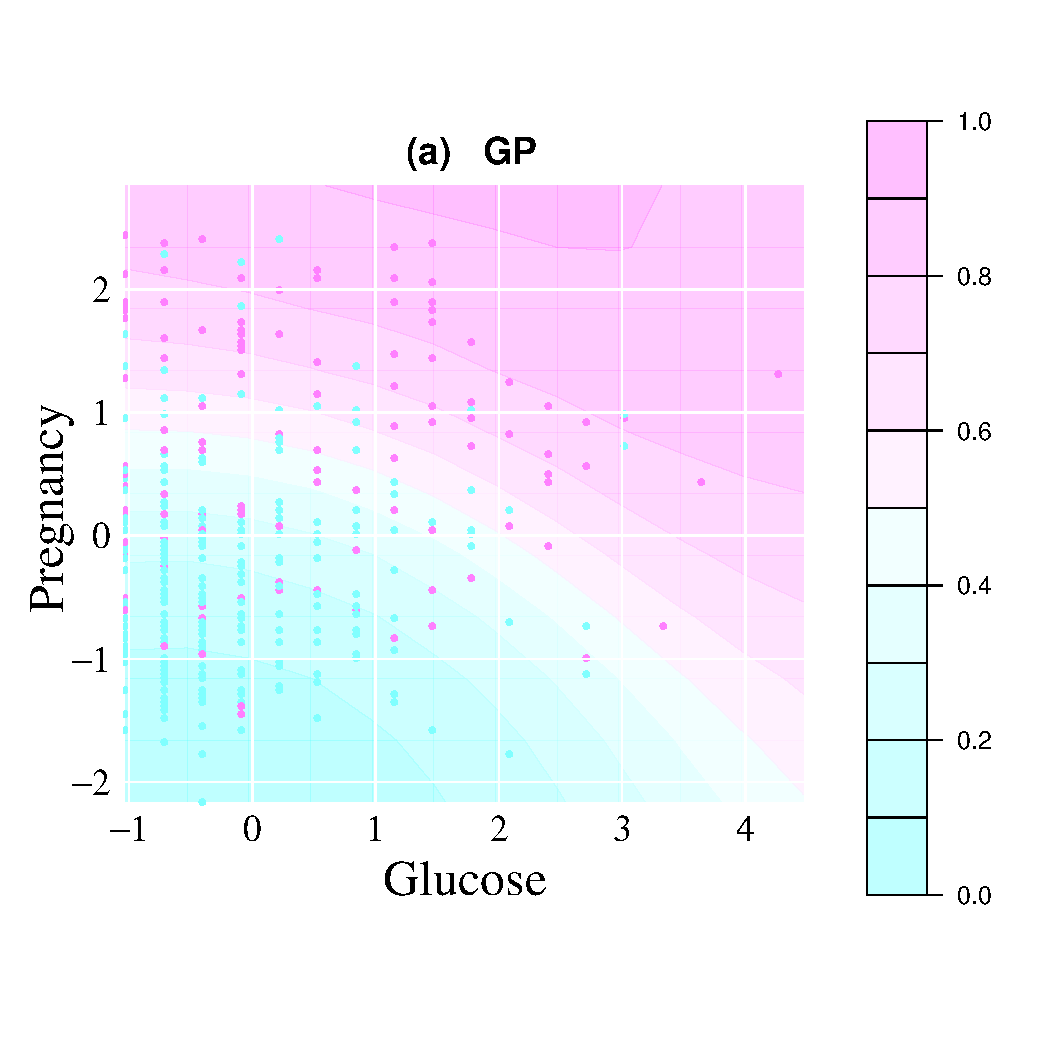
\includegraphics[scale=0.37, trim = 5mm 23mm 39mm 20mm, clip]{ch5_fig18_gpfun_diabetes.pdf}}
\subfigure{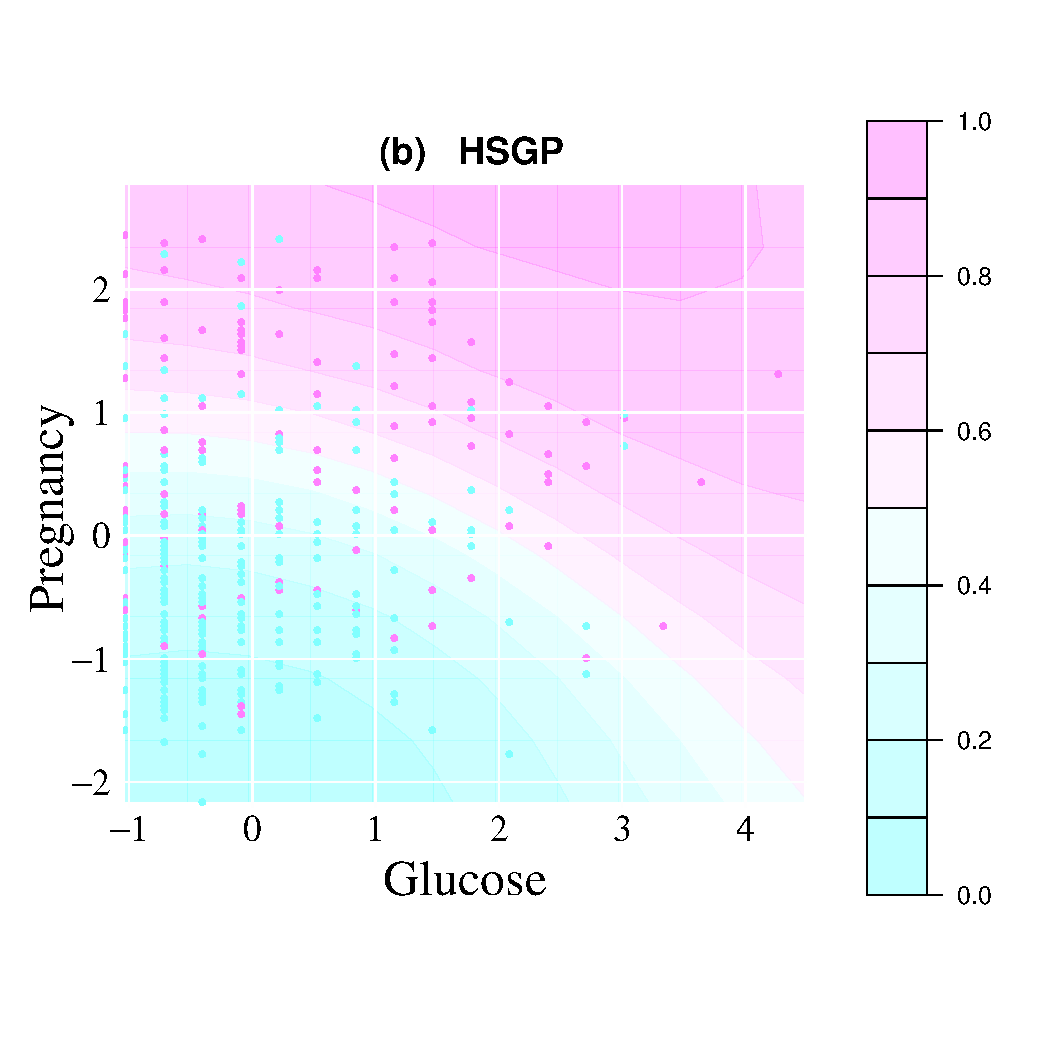
\includegraphics[scale=0.37, trim = 20mm 23mm 39mm 20mm, clip]{ch5_fig18_bffun_diabetes.pdf}}
\subfigure{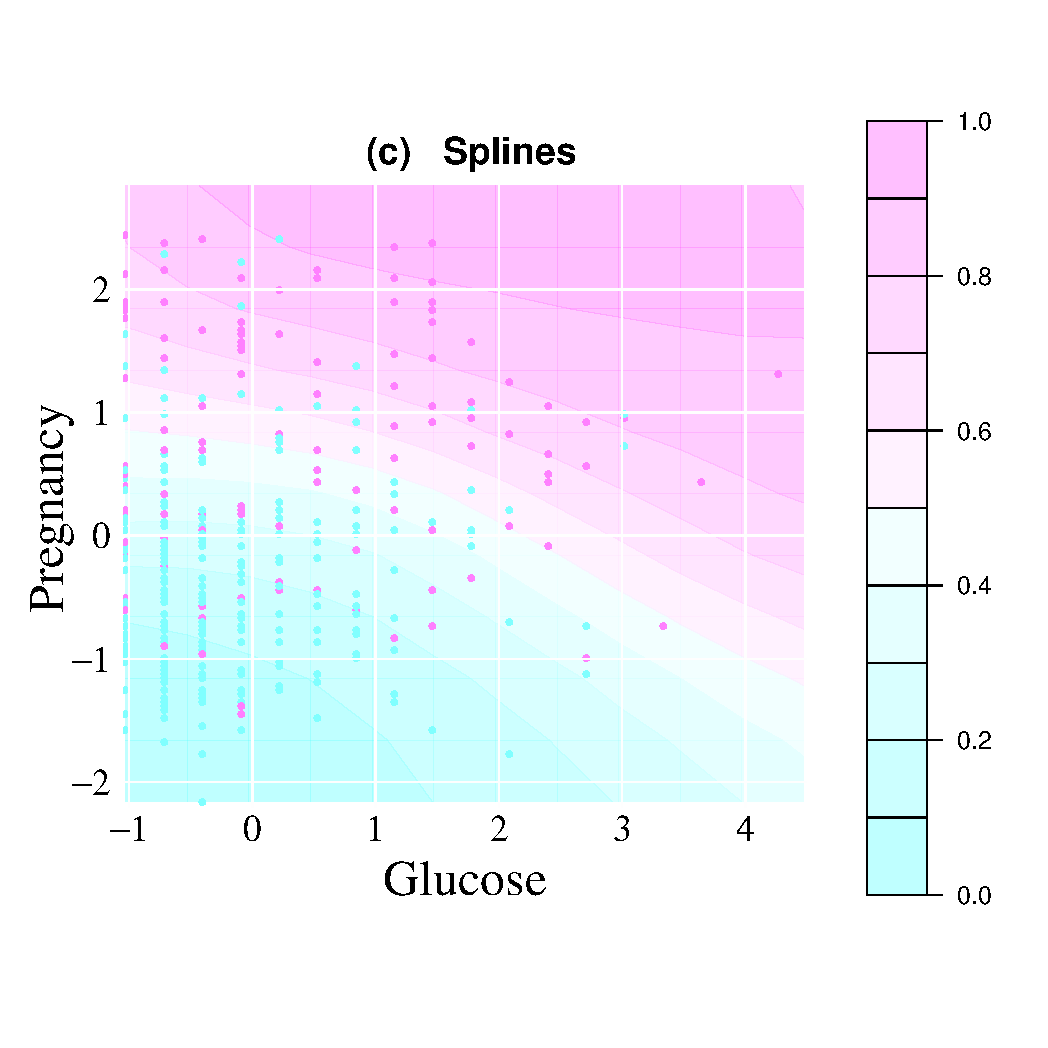
\includegraphics[scale=0.37, trim = 20mm 23mm 39mm 20mm, clip]{ch5_fig18_spfun_diabetes.pdf}}
\subfigure{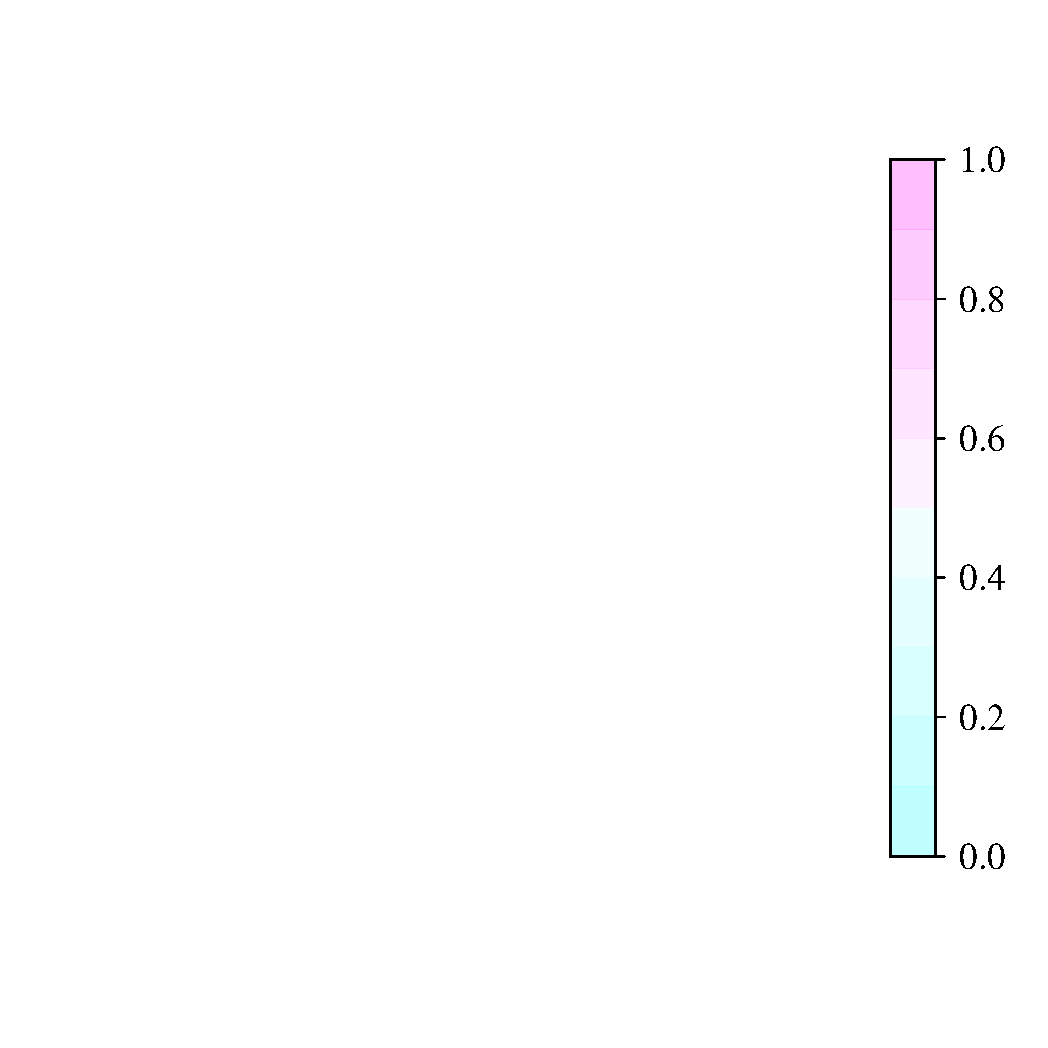
\includegraphics[scale=0.30, trim = 150mm 4mm 2mm 15mm, clip]{ch5_fig18_legend_diabetes.pdf}}
\caption{(a) Mean posterior predictive functions of the GP model. (b) Mean posterior predictive functions of the HSGP model. (c) Mean posterior predictive functions of the spline (SP) model. Samples observations of suffering (red points) and not suffering (blue points) form the disease are plotted.}
  \label{ch5_fig18_gpfun_diabetes}
\end{figure}

In order to assess the performance of the models as a function of the boundary factor, the number of basis functions and knots, different models with different number of basis functions and boundary factor for the HSGP model and different number of knots for the spline model have been fitted. In all models, the same boundary factor, number of basis functions and knots per dimension were used. Figure \ref{ch5_fig19_ELPD_diabetes} shows the expected log predictive density (ELPD; see \cite{vehtari_2012}) as a function of the boundary factor $c$ and the number of univariate basis functions $m$, for the HSGP model, and knots, for the spline model. The ELPD is computed over the actual observations by cross-validation. Basically, with slightly differences, all models show similar performances, due to the fact that the process is very smooth with a relatively very large lengthscale estimate $\ell=4.51$. Even though, a slight pattern of performance improvement can be appreciated as the boundary factor $c$ increases, which fact is because small boundary factors are not allowed when large lengthscales (Figure 6% \ref{fig6_lscale_vs_J_vs_c}
).
%
\begin{figure}
\centering
\subfigure{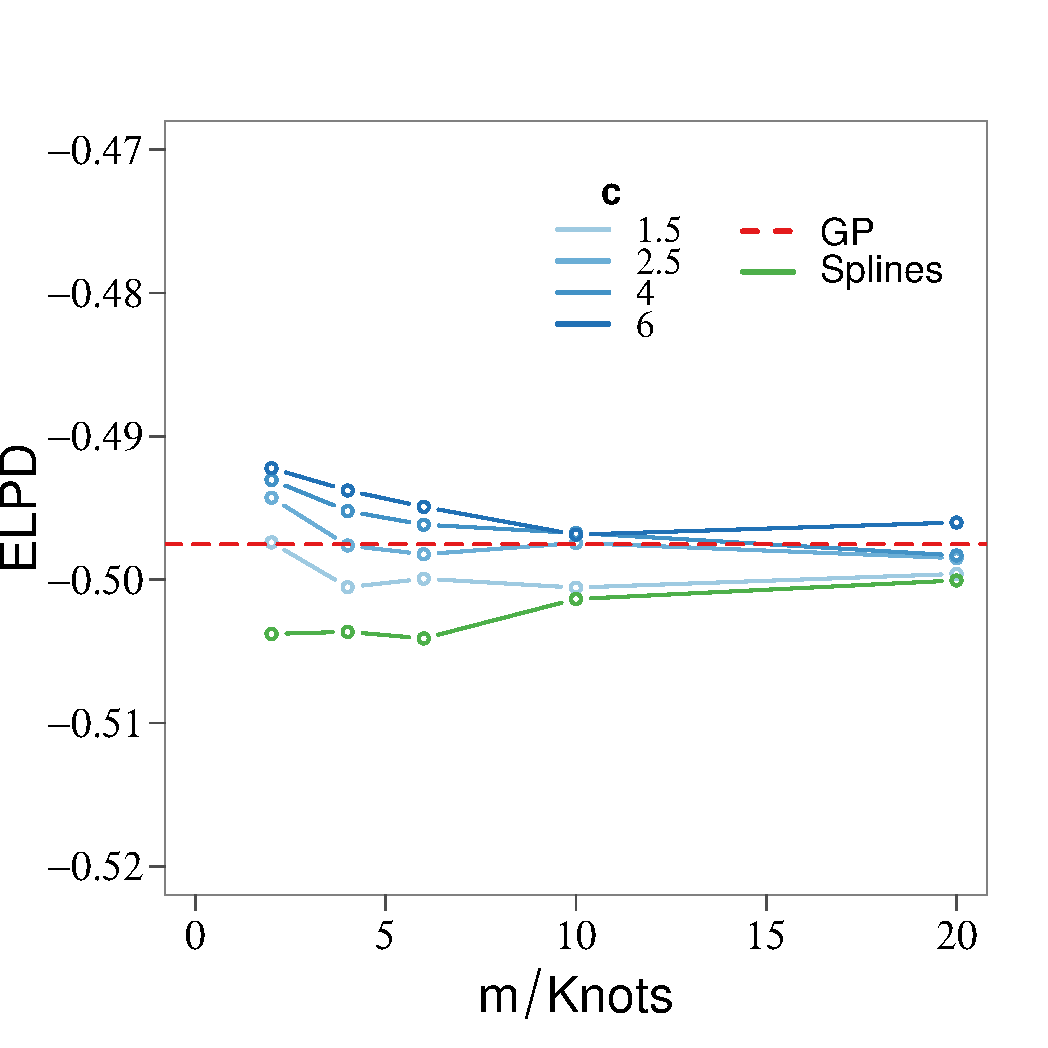
\includegraphics[scale=0.38, trim = 0mm 0mm 10mm 0mm, clip]{ch5_fig19_ELPD_diabetes.pdf}}
\caption{Expected log predictive density (ELPD) of the different methods as a function of the boundary factor $c$ and the number of basis functions $m$, for the HSGP model, and knots, for the spline model.}
  \label{ch5_fig19_ELPD_diabetes}
\end{figure}

Figure \ref{ch5_fig20_time2D_diabetes} shows the computational times of the different models, regular GP, HSGP and spline, fitted over the dataset with 2, 3 and 4 input dimensions, as a function of the boundary factor $c$ and number of univariate basis functions $m$ and knots. The time of omputation increases significantly with higher dimensions for the HSGP and spline models. In this sense, choosing optimal values for the number of basis functions and boundary factor, looking at the recommendations and diagnosis provided by Figure 6 % \ref{fig6_lscale_vs_J_vs_c}
in the main document, can be essential to avoid a excessive computation time, especially in multivariate input spaces. Serious difficulties with computation time were encountered in building spline models in a 4D input space or even in a 3D input space with more than 10 knots.

The Stan model codes for the exact GP, the approximate GP and the spline models of this case study can be found online at {\small \url{https://github.com/gabriuma/basis_functions_approach_to_GP/tree/master/Paper/Case-study_Diabetes-data}}.

\begin{figure}
\centering
\subfigure{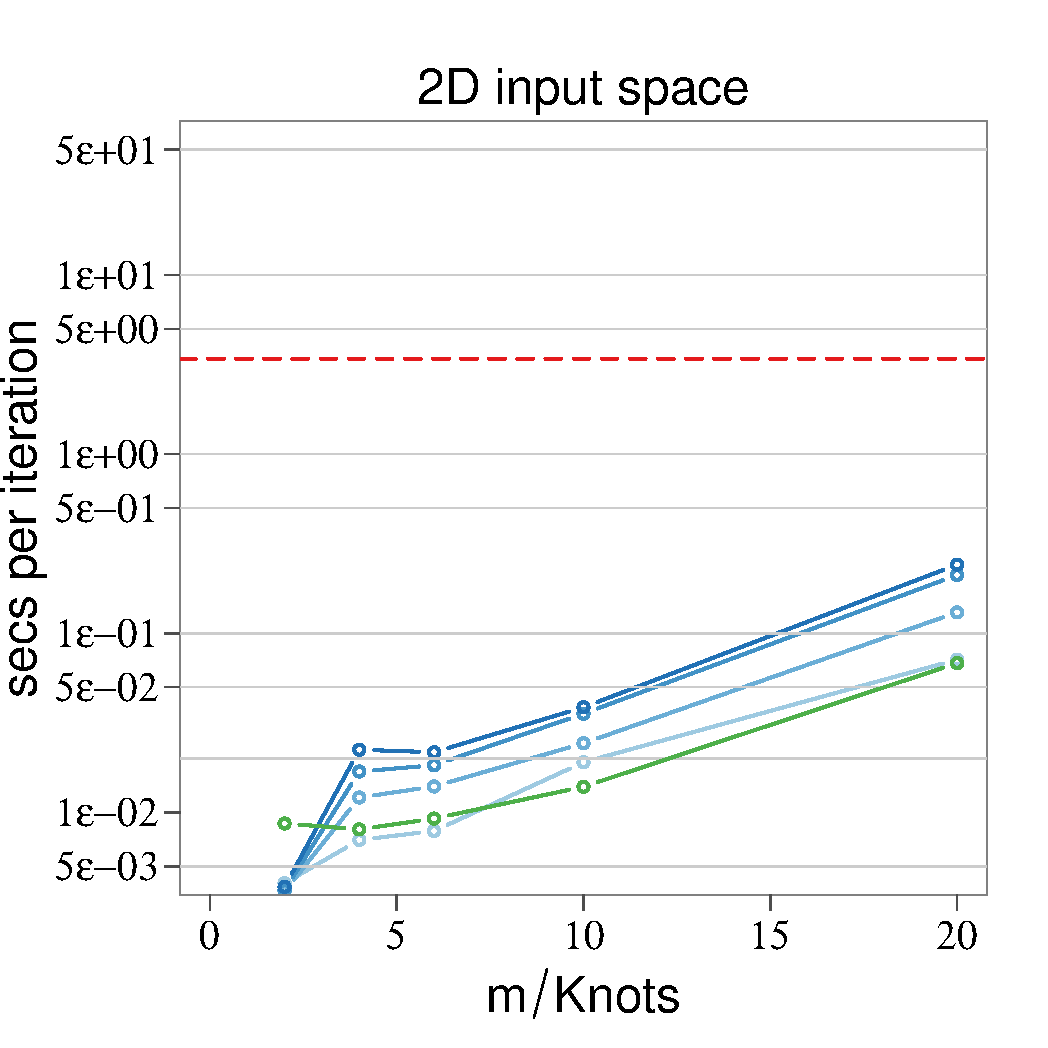
\includegraphics[scale=0.29, trim = 1mm 0mm 10mm 0mm, clip]{ch5_fig20_time2D_diabetes_2.pdf}}
\subfigure{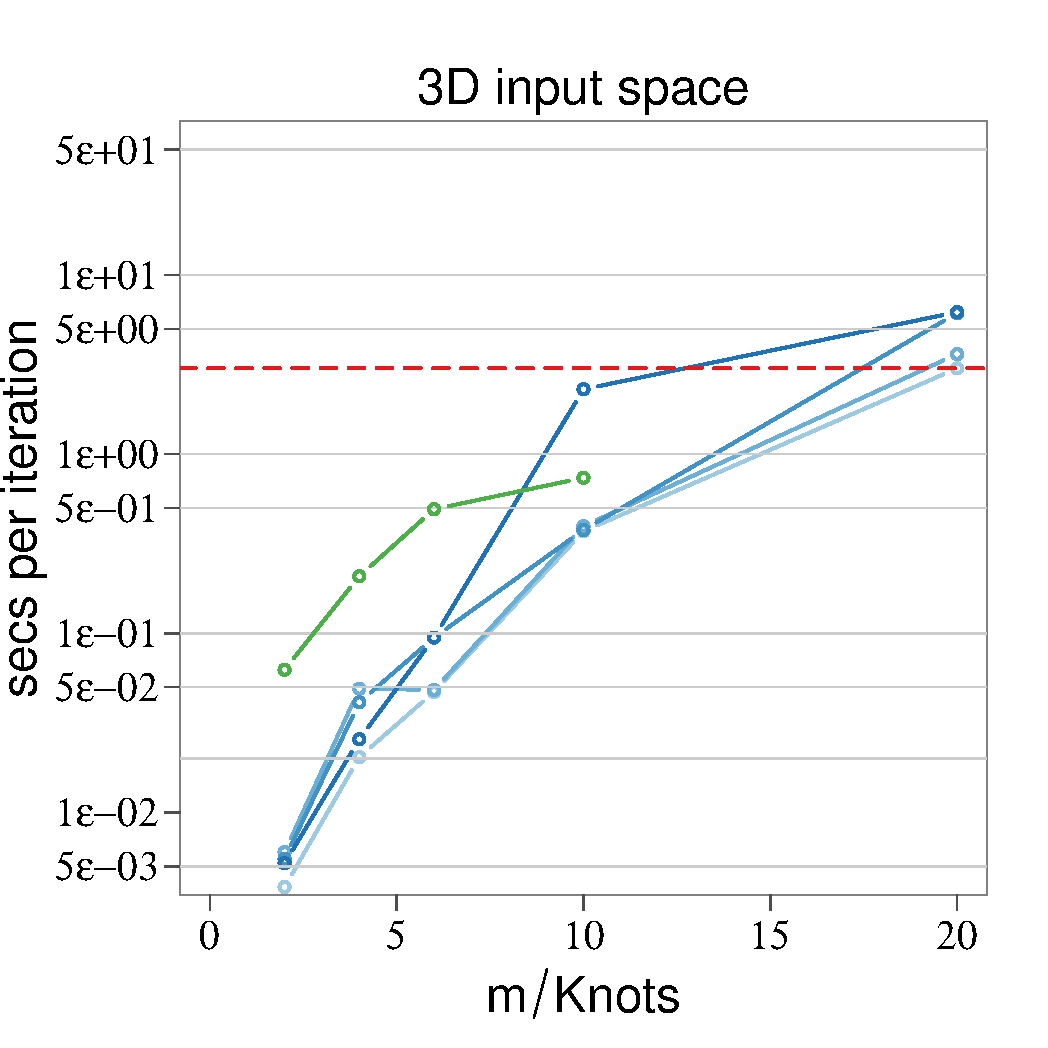
\includegraphics[scale=0.29, trim = 30.2mm 0mm 10mm 0mm, clip]{ch5_fig20_time3D_diabetes_2.pdf}}
\subfigure{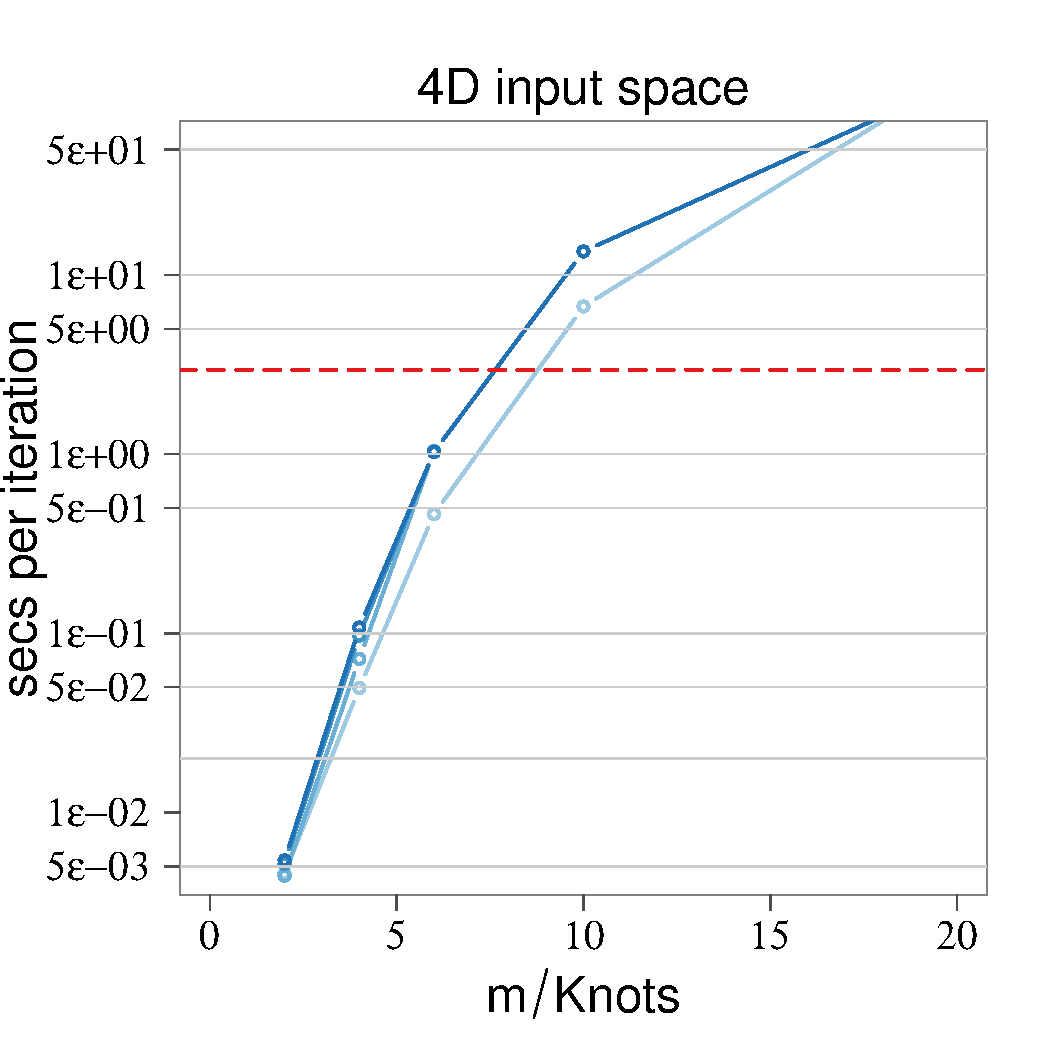
\includegraphics[scale=0.29, trim = 30.2mm 0mm 10mm 0mm, clip]{ch5_fig20_time4D_diabetes_2.pdf}}
\subfigure{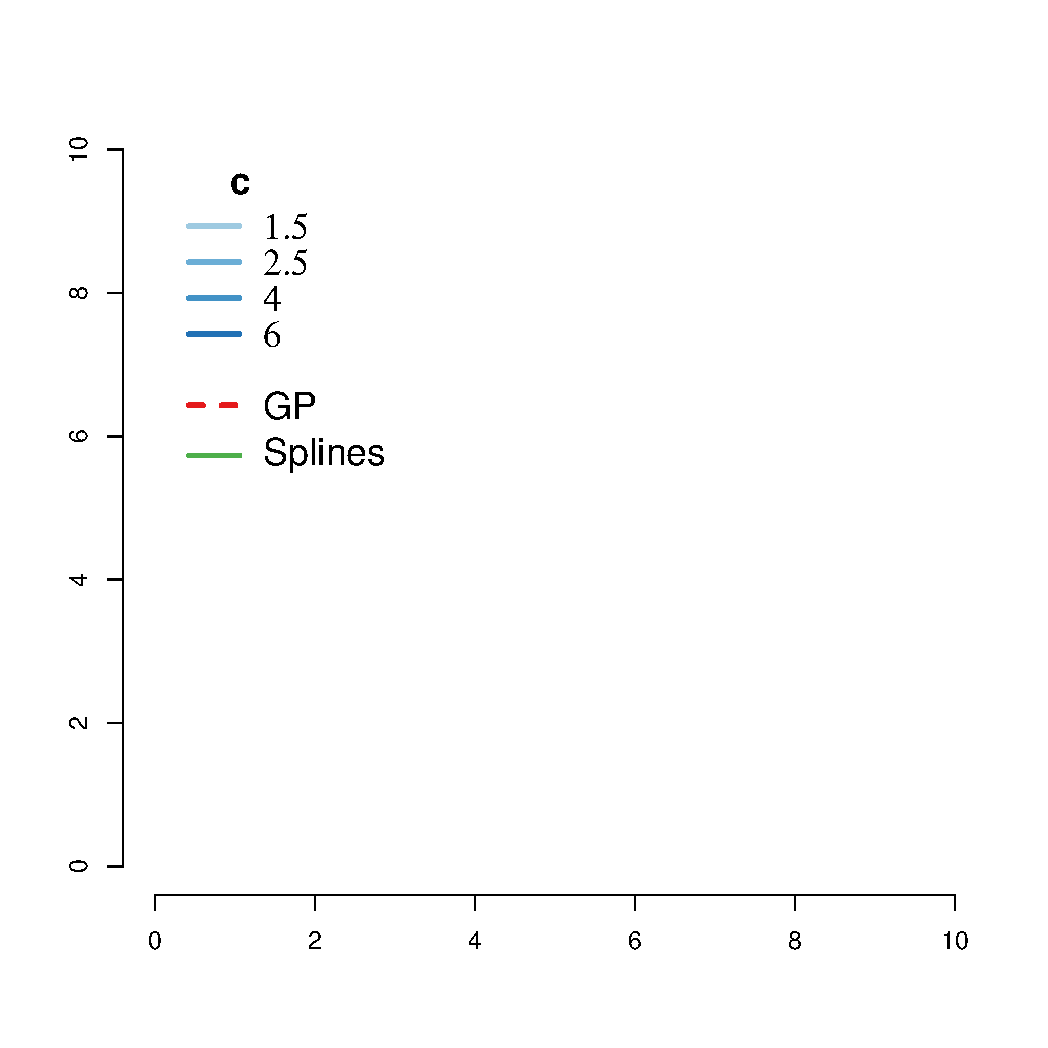
\includegraphics[scale=0.35, trim = 28mm 50mm 112mm 10mm, clip]{ch5_fig20_legend_diabetes_2.pdf}}
\caption{Time of computation in seconds per iteration (iteration of the HMC sampling method) of the different models fitted over the dataset, with 2 input dimensions (left) and 3 input dimensions (center) and 4 input dimensions (right), as a function of the boundary factor $c$ and number of basis functions $m$, for the HSGP model, and knots, for the spline model. The y-axis is on a logarithmic scale.}
  \label{ch5_fig20_time2D_diabetes}
\end{figure}


\section{Spatio-temporal land-use classification case study}\label{ch5_sec_application_caseII}


The next example presents an spatio-temporal classification in land-use of plots between 2006 and 2015 in a part of the territory of Valencia in Spain dedicated to growing citrus fruits. A sampling set consists of $n=200$ plots with known class. The data is recorded in a time series of $T=5$ years (2006, 2008, 2010, 2012, 2015) within the period. The class of each parcel $i$ and time $t$ is stored by a categorical variable $y_{it}$ representing the $K=5$ different possible classes ($k=1,\dots,K$): $k=1$, adult independent citrus fruits; $k=2$, aligned citrus fruits; $k=3$, irregular citrus fruits; $k=4$, abandoned citrus fruits; $k=5$, young citrus fruits. 

A bunch of 52 characteristic variables was available for every parcel and time. These variables were computed from satellite color images and cadastral map by using the software FETEX for automatic descriptive feature extraction from image-objects \citep{ruiz2011feature}. These variables concern spectral intensities and empirical semivariogram of the pixels within a plot, as well as descriptive statistics of the shape of the plots.

Due to the fact that 52 input variables are too high-dimensional for a multivariate HSGP model, which computational cost scales as $O(n m^D+m^D)$, with $m$ the number of basis functions and $D$ the number of input variables, the multivariate HSGP model will be formulated as an additive HSGP model. 

As it is known, the computational demand of a multivariate HSGP model component increases quickly with the number of dimensions, so we should avoid high-dimensional HSGP components in the additive model. Original input variables are highly correlated, which would imply the use of high-order interaction components in the additive model to achieve accurate model performance. Therefore, instead of using the original variables as inputs, we use their principal components, which are expect to be linearly uncorrelated. Using the principal components as inputs helps, in principle, not to have to use as many high-order interaction components in the additive model.  

The principal components (PCs) will be used jointly with the time variable as inputs in the classifying additive HSGP model. Let's denote the matrix $\bm{X}=[\bm{x}_{11}\, \cdots \, \bm{x}_{it} \, \cdots \, \bm{x}_{nT}]^\top \in {\rm I\!R}^{nT\times D}$, which contains the input vectors $\bm{x}_{it} \in {\rm I\!R}^D$, $D=53$ ($52 \text{ PCs plus time}$) for the spatio-temporal observations (plots $i=1,\dots,200$, and times $t=1,\dots,5$). 

The observational model is a multinomial model with parameters the vector of probabilities $\bm{p}_{it}=(p_{it,1},p_{it,2},\dots,p_{it,K})$, where $p_{it,k}$ is the probability of belonging to class $k$ per parcel $i$ and time $t$,
%
\begin{equation*}
y_{it} \sim \mathrm{Multinomial}(\bm{p}_{it}).
\end{equation*}

\noindent The goal is to estimate the vector of probabilities $\bm{p}_{it}$ as a function of the predictors, which is a multivariate function $f(\bm{x}_{it}):{\rm I\!R}^{D} \rightarrow {\rm I\!R}^{K}$,
$$
f(\bm{x}_{it})=\big(f_1(\bm{x}_{it}),\dots,f_K(\bm{x}_{it}) \big),
$$

\noindent which is related to the vector of probabilities $\bm{p}_{it}$ through the 'softmax' link function:
%
\begin{equation*}
\bm{p}_{it} = \mathrm{softmax}(f(\bm{x}_{it})).
\end{equation*}

Each individual function $f_k(\bm{x})$ is modeled as a first-order additive model plus the second-order additive effects between time input variable ($x^D$) and all the other inputs as follows: 
%
\begin{equation} \label{ch5_eq_f_parcels}
f_k(\bm{x}) = \sum_{d=1}^{D} g_d(x^d) + \sum_{d=1}^{D-1} h_{d,D}(x^d,x^D).
%\mathcal{HSGP}(x^d, S(\bm{\lambda}), \theta_d),
\end{equation}

\noindent The first-order components $\{g_d(x^d)\}_{d=1}^D$ in equation (\ref{ch5_eq_f_parcels}) are modeled as unidimensional HSGP models:
%
\begin{equation*}
g_d(x^d) \sim \mathcal{HSGP}(x^d, S, \theta_{d,1}).
\end{equation*}

\noindent In the HSGP model, a first-order components $g_d(x^d)$, evaluated at input value $x^d \in {\rm I\!R}$, is approximated as in equation (7) % (\ref{eq_approxf}) 
with the squared exponential spectral density $S$ as in equation (1) % (\ref{eq_specdens_inf})
 and eigenvalues $\lambda_j$  and eigenfunctions $\phi_j$ as in equations (5) % (\ref{eq_eigenvalue})
and (6)% (\ref{eq_eigenfunction})
  , respectively. 

The second-order components $\{h_{d,D}(x^d,x^D)\}_{d=1}^{D-1}$ in equation (\ref{ch5_eq_f_parcels}) are modeled as two-dimensional HSGP models:
%
\begin{equation*}
h_{d,D}(x^d,x^D) \sim \mathcal{HSGP}(x^d,x^D, S, \theta_{d,D}).
\end{equation*} 

\noindent In the HSGP model, a second-order component $h_{d,D}(x^d,x^D)$, evaluated at inputs $x^d \in {\rm I\!R}$ and $x^D \in {\rm I\!R}$, is approximated as in equation (12)% (\ref{eq_approxf_multi})
 with the two-dimensional (with a scalar lengthscale) squared exponential spectral density $S$ as in equation (1) % (\ref{eq_specdens_inf}) 
 and the $D$-vector of eigenvalues $\bm{\lambda}_j$ and the multivariate eigenfunctions $\phi_j$ as in equations (9) % (\ref{eq_eigenvalue_multi}) 
 and (10)% (\ref{eq_eigenfunction_multi})
 , respectively. 

The vector of hyperparameters $\theta_{d,1}=(\alpha_{d,1},\ell_{d,1})$ contains the marginal variance $\alpha_{d,1}$ and lengthscale $\ell_{d,1}$ of the $g_d(x^d)$ model component. And, the vector of hyperparameters $\theta_{d,D}=(\alpha_{d,D},\ell_{d,D})$ contains the marginal variance $\alpha_{d,D}$ and lengthscale $\ell_{d,D}$ of the $h_{d,D}(x^d,x^D)$ model component.
 

For the first-order components $g_d(x^d)$, $m=15$ basis functions and a boundary factor $c=2.5$ were used. For the second-order components $h_{d,D}(x^d,x^D)$, $m_1=15$ and $m_2=15$ basis functions for each dimension, respectively, were used, which lead to a total of 225 multivariate basis functions. A boundary factor for each dimension $c_1=2.5$ and $c_2=2.5$ were used. All the input variables were previously standardized.

In the case of the first-order components, the normalized lengthscale estimates $\left(\frac{2\cdot \hat{\ell}_{d,1}}{|x^d_{max}-x^d_{min}|}\right)$ are all bigger than the minimum lengthscale reported by Figure (6) % \ref{fig6_lscale_vs_J_vs_c} 
as a function of $m$ and $c$. Which means that the used number of basis functions ($m=15$) and boundary factor ($c=2.5$) are suitable values for modeling accurately the input effects.

For the second-order components, the relationships between the number of basis functions, the boundary factor and the lengthscale is not available for the multivariate case. However, we can approximately analyze the lengthscale estimates of the second-order HSGP components analyzing each dimension separately as unidimensional HSGP models.

Table \ref{ch5_tab_parcels} shows the confusion matrix after fitting the model following a $Q$-fold cross-validation procedure, with $Q=100$, over the training data. Thus, every fold contains $10$ observations. The confusion matrix evaluates the rate of misclassification per class. Columns represent the true classes and rows represent the estimated classes. The values within the matrix correspond to the number of items that fall into every cell. 
The marginals of the columns (true classes) represent the percentage of misclassified items in relation to the 'truth', commonly known as the \textit{omission error}. And the marginals of the rows (estimated classes) represent the percentage of misclassified items in relation to the estimates (classifier), commonly known as the \textit{commission error}. The percentage in the down right cell of the matrix is the overall mean misclassification rate. As can be seen, there exist a high misclassification rate between classes $k=1$ and $k=2$, between classes $k=1$ and $k=3$, and between classes $k=1$ and $k=5$.

\begin{table}
\begin{center}
\begin{tabular}{|c|*{6}{c|}}\hline
\backslashbox{\small Estimate}{\small True} & \multicolumn{1}{p{1cm}|}{\centering k = 1} &  \multicolumn{1}{p{1cm}|}{\centering k = 2} & \multicolumn{1}{p{1cm}|}{\centering k = 3} & \multicolumn{1}{p{1cm}|}{\centering k = 4} & \multicolumn{1}{p{1cm}|}{\centering k = 5} & \multicolumn{1}{p{1cm}|}{\centering } \\ 
\hline \multicolumn{1}{|p{3cm}|}{ \centering k = 1} &90&39&14&3&11&42\%\\
\hline \multicolumn{1}{|p{3cm}|}{\centering k = 2} &46&301&8&2&3&16\%\\
\hline \multicolumn{1}{|p{3cm}|}{\centering k = 3}  &8&4&59&4&1&19\%\\
\hline \multicolumn{1}{|p{3cm}|}{\centering k = 4}  &5&2&6&342&5&5\%\\
\hline \multicolumn{1}{|p{3cm}|}{\centering k = 5}  &8&2&1&0&38&19\%\\
\hline \multicolumn{1}{|p{3cm}|}{\centering }  &42\%&13\%&32\%&2\%&34\%&$\textbf{17\%}$\\
\hline
\end{tabular}
\end{center}
\caption{Confusion matrix after the Q-fold cross-validation procedure over the training data.}
  \label{ch5_tab_parcels}
\end{table}

The Stan model code for the approximate GP model of this case study can be found at {\small \url{https://github.com/gabriuma/basis_functions_approach_to_GP/tree/master/Paper/Case-study_Land-use-classification}}.


\bibliography{references}

\end{document}


